%%%%%%%%%%%%%%%%%%%%%%%%%%%%%%%%%%%%%%%%%%%%%%%
%
% Template per Elaborato di Laurea
% DISI - Dipartimento di Ingegneria e Scienza dell’Informazione
%
% update 2015-09-10
%
% Per la generazione corretta del 
% pdflatex nome_file.tex
% bibtex nome_file.aux
% pdflatex nome_file.tex
% pdflatex nome_file.tex
%
%%%%%%%%%%%%%%%%%%%%%%%%%%%%%%%%%%%%%%%%%%%%%%%

% formato FRONTE RETRO
\documentclass[epsfig,a4paper,11pt,titlepage,twoside,openany]{book}
\usepackage{epsfig}
\usepackage{plain}
\usepackage{setspace}
\usepackage[paperheight=29.7cm,paperwidth=21cm,outer=1.5cm,inner=2.5cm,top=2cm,bottom=2cm]{geometry} % per definizione layout
\usepackage{titlesec} % per formato custom dei titoli dei capitoli

\usepackage{graphicx}
\graphicspath{ {./images/} }
\usepackage{algorithm}
\usepackage{algpseudocode}
\usepackage{amsmath}
\usepackage{algorithm}
\usepackage{url}
\usepackage{hyperref}
\usepackage{caption}
\usepackage{subcaption}

\begin{document}

  % nessuna numerazione
  \pagenumbering{gobble} 
  \pagestyle{plain}

\thispagestyle{empty}

\begin{center}
  \begin{figure}[h!]
    \centerline{
\psfig{file=marchio_unitrento_colore_it_202002.eps,width=0.6\textwidth}}
  \end{figure}

  \vspace{2 cm} 

  \LARGE{Department of Information Engineering and Computer Science\\}

  \vspace{1 cm} 
  \Large{Bachelor’s Degree in\\
    Computer, Communication ad Electronic Engineering
  }

  \vspace{2 cm} 
  \Large\textsc{FINAL DISSERTATION\\} 
  \vspace{1 cm} 
  \Huge\textsc{Promoting Quality Diversity in Soft Robot co-design evolution\\}


  \vspace{2 cm} 
  \begin{tabular*}{\textwidth}{ c @{\extracolsep{\fill}} c }
  \Large{Supervisor} & \Large{Student}\\
  \Large{Prof. Giovanni Iacca}& \Large{Elisa Composta}\\
  \Large{Co-supervisor}&\\
  \Large{Andrea Ferigo}
  \end{tabular*}

  \vspace{2 cm} 

  \Large{Academic year 2021/2022}
  
\end{center}


  \clearpage
 
  \thispagestyle{empty}

\begin{center}
  {\bf \Huge Acknowledgements}
\end{center}

\vspace{4cm}

\emph{\\
I would like to thank Prof. Iacca and Andrea for guiding me with patience and dedication in these months, from the beginning of the project till the realization of this work.\\
I am also extremely grateful to my family, for always supporting me and believing in all of my choices.\\
Special thanks to Simone, by my side since the very first day of this journey, with whom I shared the hardest times, the best moments, and all of my dreams.\\
I would like to extend my sincere thanks to the people I met in these last years, especially my project teammates, for encouraging my personal growth by providing me differing perspectives.}


  \clearpage
  \pagestyle{plain} % nessuna intestazione e pie pagina con numero al centro

  % inizio numerazione pagine in numeri arabi
  \mainmatter

    % indice
    \tableofcontents
    \clearpage

    % gruppo per definizone di successione capitoli senza interruzione di pagina
    \begingroup
      % nessuna interruzione di pagina tra capitoli
      % ridefinizione dei comandi di clear page
      \renewcommand{\cleardoublepage}{} 
      \renewcommand{\clearpage}{} 
      % redefinizione del formato del titolo del capitolo
      % da formato
      %   Capitolo X
      %   Titolo capitolo
      % a formato
      %   X   Titolo capitolo
      
      \titleformat{\chapter}
        {\normalfont\Huge\bfseries}{\thechapter}{1em}{}
        
      \titlespacing*{\chapter}{0pt}{0.59in}{0.02in}
      \titlespacing*{\section}{0pt}{0.20in}{0.02in}
      \titlespacing*{\subsection}{0pt}{0.10in}{0.02in}
      
      % abstract
      \chapter*{Abstract} % senza numerazione
\label{abstract}

\addcontentsline{toc}{chapter}{Abstract} % da aggiungere comunque all'indice

An important and promising robotic subject that is gaining ground is Soft Robotics, a sub-field that examines robots with a soft and deformable body.\\
What makes these individuals so powerful, is that their malleable morphology allows them to face complex and dynamic environments and gives them the chance to perform well even on the hardest tasks.\\
This is a promising area, since it will enhance human-machine interaction, having many future bio-related applications, like prostheses, artificial organs, and support for gait rehabilitation.
However, it sets many challenges due to the complexity of finding individuals that are both soft and robust, able to adapt to unpredictable environments, therefore it requires deeper studies.

Robots, just like living creatures, should be a good match of body and brain.
It's easy to imagine that some bodies are intrinsically better than others: an individual with two flexible legs walks better than a rigid squared box.
Another simple and intuitive idea is that the brain certainly plays an equally important role: what is a body without a brain?
Even the best bodies can have poor results, having no control of their actions.\\
Given this premises, it is evident that body and brain must be both optimized, in order make individuals perform their best.
However, while many researches focus on the controller optimization, less attention is placed on finding the best bodies, mainly because the co-optimization of body and brain is still a challenging problem.

This work addresses the co-optimization problem of soft robots using Reinforcement Learning to optimize the controller and applying Evolutionary Algorithms to design morphologies.\\
It presents the importance of co-designing both the body and the controller and it makes a comparison between two existing evolutionary algorithms, MAP-Elites and the Genetic Algorithm.\\
A focus on the controller optimization highlights its role in improving the performances, since it allows also disadvantaged body to perform their best.

An analysis on the adaptability of individuals was made by evaluating them in environments they have not been trained for, optimizing the controller in the new task.

Even though this work only provides an overview of soft robot evolution, what emerges is that this is a promising field, and further studies might lead to interesting results, with many possible future applications.




      \newpage
      
      % lista dei capitoli
      \chapter{Introduction}
\label{cha:chapter1}

Soft robotics is a research field that evolves robots with a soft and deformable body, which guarantees them flexibility and adaptability, allowing them to face complex and unpredictable environments: for instance, they can perform smooth locomotion on rough terrain~\cite{8460667}, or squeeze through tight spaces~\cite{10.1145/2739480.2754662}

To find optimal individuals it's important to optimize both the bodies and the controllers.\\
It's clear that some individuals are intrinsically better than others at some tasks, only because of their morphology; for example, a robot with two legs surely walks better than a rigid squared box.\\
This intuitive concept is the basis of Embodied Intelligence, theory that states that the body of an agent plays a fundamental role in simplifying tasks and in making adaptive behaviours emerge through the interaction with the environment~\cite{Cianchetti2021}.\\
At the same time the controller, which is the brain telling the robot which action to take, has a key role, since it determines the behaviour of the individual in the environment.\\
For these reasons, it's important to optimize both the body and the controller of the robots, in order to find fitting morphologies with proper behaviours.

However, many existing studies focus on the controller optimization, but little attention is placed on finding the optimal bodies.
This is mainly because co-optimizing the body and the controller in robotics is characterized as a challenging problem~\cite{bhatia2021evolution}.

What makes soft robots interesting is their flexibility and softness, which makes them ideal for many future bio-related applications, since it promises an enhanced human-machine interaction.\\
They have been proposed as a support for gait rehabilitation~\cite{6696468} and colonoscopies~\cite{Zhang2019-fm}, and some other possible future applications are artificial organs and tissue-mimicking active simulators for training and biomechanical studies~\cite{Cianchetti2018}.

This work proposes soft robot co-evolution by combining two main libraries: Evolution Gym~\cite{evogym}, that provides the simulator, the co-optimization structure, the tasks to work on and an implementation of GA, and QDpy~\cite{qdpy}, for the MAP-Elites algorithm implementation, adjusted to work on soft robot evolution.

This chapter is intended to provide the basic notions of the topics related to this work, including how soft robots differ from conventional rigid robots, an overview on the algorithms used and the benchmark adopted.
The second chapter focuses on the importance of optimizing the controller, while a comparison of body optimization algorithms, MAP-Elites and GA, is proposed in the following chapter.
An analysis on how individuals behave in different environments is introduced in the fourth chapter.
Finally, the conclusions provide an overview of what emerged from the experiments presented and introduce some possible future works.


%%% SOFT ROBOTS %%%
\section{Soft Robots}
Conventionally, engineers have employed rigid materials to fabricate precise, predictable robotic systems, which are easily modelled as rigid members connected at discrete joints.\\
Rigid-bodied robots can be efficient on a single task, however they don't easily adapt to the environment.
What is more, they are often unsafe for interaction with humans.\\
A solution might be provided by soft robotics, research field that aims at evolving robots with a deformable structure and muscle-like actuation that emulates biological systems, yielding to adaptability and a smooth interaction with the environment~\cite{Rus2015}.

The body of each robot in Evolution Gym is composed of various types of primitive building blocks, and the control of the robot includes action signals applied on the actuator voxels.


\subsection{Body}
The soft robot evolved in this work are voxel-based, which means they are composed of primitive blocks of various type.
This multi-material voxel-based structure provides a general
and universal representation for various categories of robot designs, and at the same time results in a modular and expressive structure design space~\cite{bhatia2021evolution}.

The robot body is defined as a matrix, where each entry is an integer corresponding to a voxel type, defined in Table \ref{tab:voxel}, and a list of connections, describing the adjacent voxels. The bodies of the robots considered in this work are defined by a 5x5 matrix.
Note that a generated body is considered valid if it is connected and it has at least one actuator.

\begin{table}[h]
    \centering
    \begin{tabular}{|l|c|l|l|}
        \hline
        \textbf{Voxel type} & \textbf{Value} & \textbf{Color} & \textbf{Behaviour}\\
        \hline
        Empty & 0 & white & -\\
        Rigid & 1 & black & not deformable\\
        Soft & 2 & grey & deformable\\
        Horizontal actuator & 3 & orange & can expand/contract horizontally\\
        Vertical actuator & 4 & blue & can expand/contract vertically\\
        Fixed & 5 & black & not deformable, fixed position\\
        \hline
    \end{tabular}
    \caption{Voxel types representation}
    \label{tab:voxel}
\end{table}

Soft voxels are deformable under the action of external forces; actuators are the ones that allow the body motion thanks to their gradual expansion/contraction in one direction, according to the action provided by the controller.
No robot can be composed of fixed voxels, since they are only used in the definition of the environments to build, for example, the terrain to walk on.

The simulation converts all objects into a set of point masses and springs by turning each voxel
into a cross-braced square as shown in the blue panel of Figure \ref{fig:obj_repr}. The figure also displays the voxel graphic representations, together with a legend of the colors chosen to differentiate the voxels types.

\begin{figure}
    \centering
    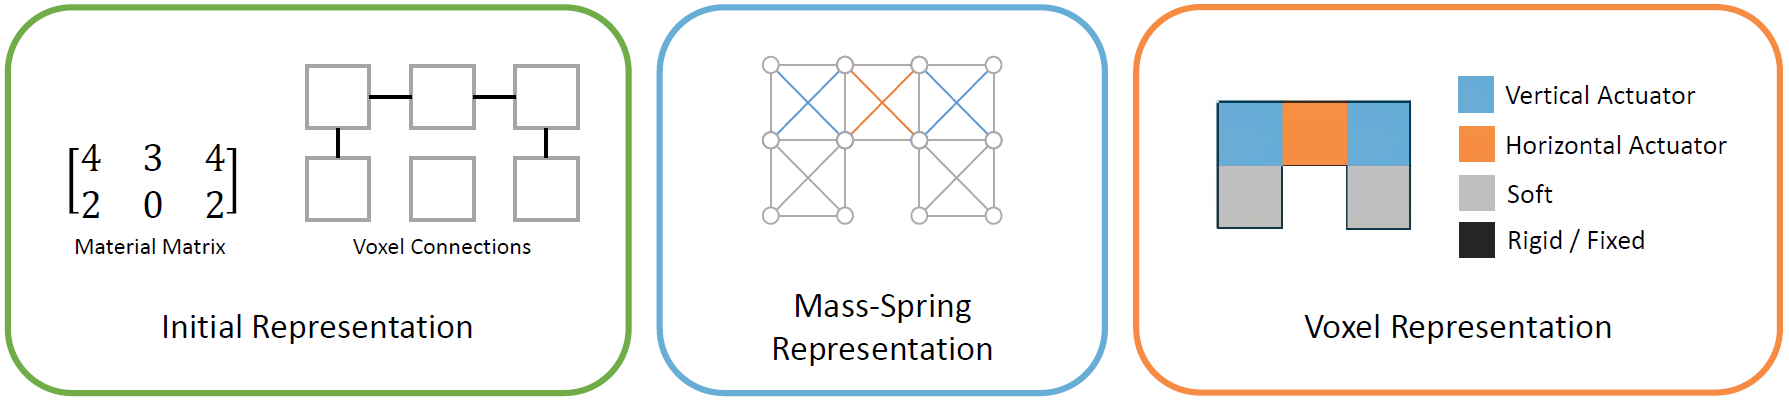
\includegraphics[scale=0.4]{images/obj_representation}
    \caption{Representation of the simulation object\cite{bhatia2021evolution}}
    \label{fig:obj_repr}
\end{figure}


\subsection{Controller}
The controller is implemented as a neural network.
It takes in input the state of the task, including observations about the robot, the environment and other task-specific information. Details about the observation space of the tasks studied in this work are provided later in this chapter.\\
The output provided by the controller is the action, a vector with length $a^r$, where $a^r$ is the number of actuators in the design of robot $r$. The action vector defines, for each actuator, its contraction/expansion value in relation to its rest length, and can vary in the range $[0.6, 1.6]$.


%%% OPTIMIZATION %%%
\section{Optimization}
Co-optimization plays a fundamental role in soft robot evolution: it's important to focus on both the body and the controller, since they both equally contribute to the performance of an individual.\\
In this work, the co-optimization applied is the one proposed by Evolution Gym, and is formulated as a two-level optimization problem~\cite{bhatia2021evolution}.\\
As shown in Figure \ref{fig:optimization}, the controller is optimized using reinforcement learning during the task simulations, and the final reward can be used by the design algorithm to determine the next morphology to work on.

As for the implementation, the design optimization is defined in the outer loop, while the inner loop focuses on control optimization, as shown in Algorithm \ref{alg:co_optimization}.\\
In this work, the controller is optimized using a reinforcement learning algorithm, PPO~\cite{kostrikov2018}, while the design optimization algorithms applied are the genetic algorithm~\cite{evogym} and MAP-Elites~\cite{qdpy}.

\begin{figure}[h]
    \centering
    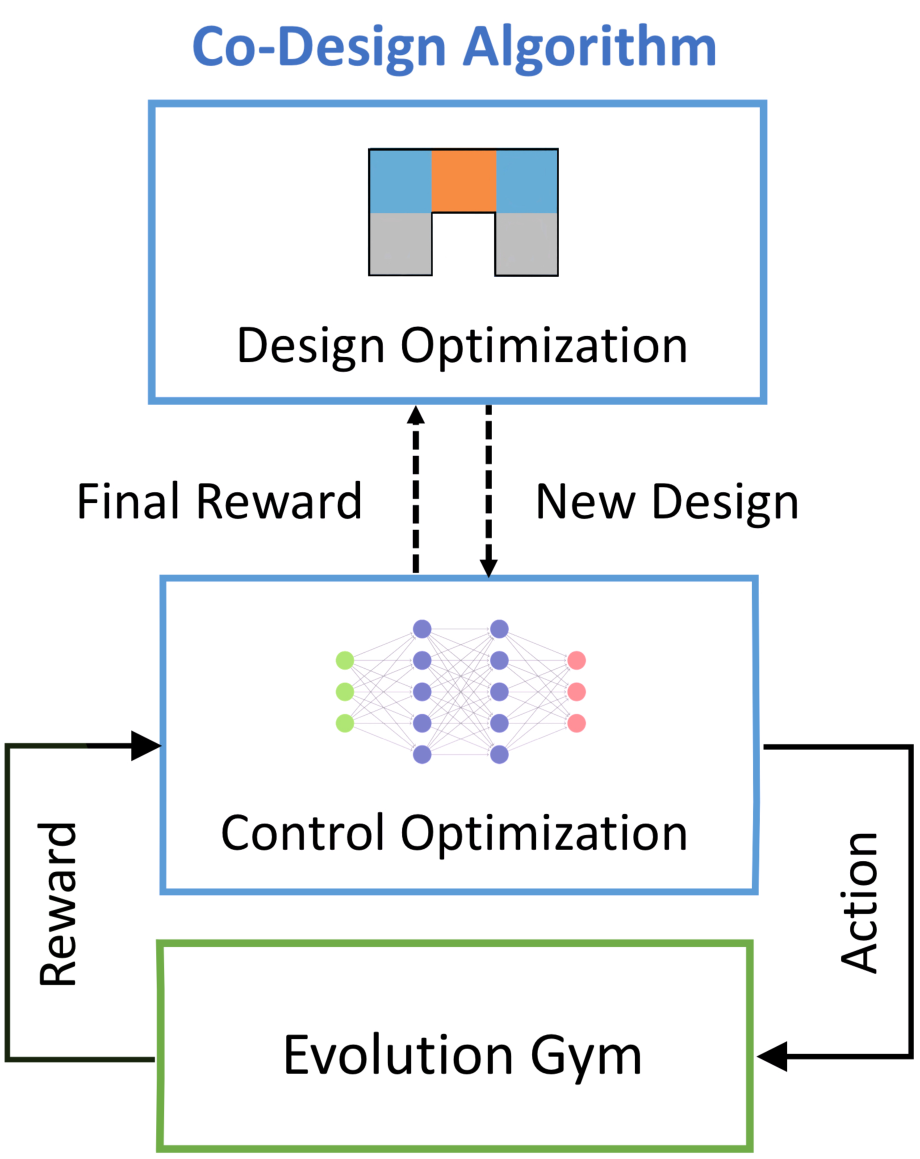
\includegraphics[scale=0.35]{images/experiment_design.pdf}
    \caption{General structure of the experiments~\cite{bhatia2021evolution}. The co-design process generates the individuals to evaluate. Evolution Gym runs the simulations according to the given bodies and controllers, and computes the reward.}
    \label{fig:optimization}
\end{figure}

\begin{algorithm}[h]
    \caption{Robot evolution co-optimization algorithm \cite{bhatia2021evolution}} \label{alg:co_optimization}
    \begin{algorithmic}
    \Require Task specification $T$, number of generations $n$, population size $p$.
        \State $S \gets \emptyset$ \hfill // Dataset of robot designs, controllers and rewards
        \State $D_1, ..., D_n \gets SampleDesigns(p)$ \hfill // Sample an initial population of robot designs
        \For{$i \gets 1$ \textbf{to} $n$}
            \For{$j \gets 1$ \textbf{to} $p$}
            \State $C_j \gets OptimizeControl(T, D_j)$ \hfill // Optimize the controller of given robot design
            \State $r_j \gets EvaluateReward(T, D_j, C_j)$ \hfill // Evaluate the reward of given design and controller
            \State $S \gets S \cup \{(D_j, C_j, r_j)\}$ \hfill // Update the evaluation result to the dataset
            \EndFor
        \State $D_1, ..., D_n \gets OptimizeDesigns(S, p)$ \hfill // Optimize a population of robot designs to evaluate
        \EndFor
    \end{algorithmic}
\end{algorithm}


\subsection{Evolutionary Algorithms}
Mainstream artificial intelligence has been very successful at designing algorithms and devices that solved stable problems. But, in doing so, in ended up neglecting fundamental aspects of biological intelligence, such as physical embodiment, behavioral autonomy, evolution and learning, that make biological organisms prone to errors and sometimes difficult to predict, but also so successful to survive in unknown and changing environments~\cite{Floreano2008}.

These premises lay out the grounding assumptions on which are founded Evolutionary Algorithms (EA): solving dynamic problems, like learning in unpredictably changing environments, requires equally dynamic solutions, that might be already provided in biology.

There are many types of EA, but the common underlying idea behind all these techniques is the same: given a population of individuals within some environment that has limited resources, competition for those resources causes natural selection (survival of the fittest)~\cite{Eiben2015}.

Applying EA to soft robot evolution has proven to be advantageous for the potential to uncover unconventional designs, difficult to anticipate for a human expert, guaranteeing efficiency and robustness.
Furthermore, evolution is able to exploit synergistic effects between body and brain that, are often too hard to model analytically.~\cite{10.1007/978-3-030-72699-7_14}

In this work two EA, introduced in the next paragraphs, are applied to soft robot design optimization: the Genetic Algorithm (GA) and the Multi-dimensional Archive of Phenotypic Elites (MAP-Elites).


\subsubsection{Genetic Algorithm}
The Genetic Algorithm (GA) is an iterative search algorithm that draws inspiration from Charles Darwin's Theory of natural selection. According to this algorithm, only the fittest individuals survive through generations. Mutation and crossover can be applied to the survivors, so as to generate offspring with more chance to fit.

The structure upon which GA are built is the following.
In each generation, the population is composed by $pop\_size$ individuals. In the first generation the designs are sampled. After the controller optimization and the evaluation, the top $x\%$  of individuals survive, and take part to the next generation. 
The survivors are iteratively sampled, and their variation, applying mutation and crossover, generates new individuals to evaluate.\\
This iterative process goes on until it meets the termination condition; in this work, the process ends when $max\_evaluations$ individuals have been evaluated.

The mutation strategy here applied states that given a morphology shape, each cell has a certain probability of mutating, defined by the \textit{mutation\_rate} parameter.
Each voxel can mutate its type into any of the others with the same probability, except for the empty type: it's three times more likely to become empty, since mutating a voxel from/to empty allows a change in the morphology. In the implementation used, no crossover has been applied.

The obtained body is considered valid if it satisfies the body constraint (being connected and having one actuator at least) and has not been already evaluated.
When the proposed body doesn't satisfy these constraints, a new mutation on the same starting individual is proposed, until the maximum number of allowed attempts, \textit{num\_attempts}, is reached.

If no valid mutated individual is found after the maximum number of attempts, it is discarded and a new body among the survivors is selected to mutate.\\


\subsubsection{MAP-Elites}
In Evolutionary Robotics a population of solutions is evolved to optimize robots that solve a given task. However, in traditional Evolutionary Algorithms, the population of solutions
tends to converge to local optima when the problem is complex or the search space is large, a problem known as premature convergence. Quality Diversity algorithms try to overcome premature convergence \cite{nordmoen2020quality} by encouraging diversity and domain illumination.

An example of QD algorithm is the Multi-dimensional Archive of Phenotypic Elites (MAP-Elites).\\
This algorithm builds a grid, where each dimension consists of a discretization of the chosen features in their domain space, according to the defined $map\_shape$.
Given the discretization, MAP-Elites searches for the highest performing solution for each cell in the N-dimensional feature space\cite{mapelites}, where N is the number of features.
Each individual is mapped to one bin only, according to its features value.
After an individual is evaluated and its features are computed, it can be inserted to the map if the corresponding bin is empty or its fitness value is greater than the one already stored, which is the occupant elite.

In the first generation, $num\_init$ individuals with randomly generated bodies are sampled, to firstly explore the map. The later generation is composed of $num\_mutated$ individuals, obtained by a mutation of bodies already evaluated and stored in the current map.\\
Individuals are evaluated in batches of size $batch\_size$.
At the end of each batch, the individuals evaluated can be inserted in the map or disregarded, as previously described.\\
The new individuals to evaluate in the next batch are generated by mutating the ones currently stored in the map.
The mutation strategy applied to these experiments is the same one used on GA, described in the previous section.\\
Note that all evaluated individuals have different morphologies since, during the experiments, evaluated bodies are hashed and stored, so as to avoid duplicated evaluations.

When all individuals are evaluated, the map represents the best individuals for each combination of features, and diversity is promoted, since different cells map to individuals with different feature values.

The features implemented and used in this work are the actuation and the emptiness of the body, described in detail in the following paragraphs.

\paragraph{Actuation}
Since Evolution Gym allows the distinction of voxel types, it's possible to define a feature that considers the number of actuators, which allow the robot motion.\\
The actuation $A$ used in these experiments is defined as follows:
\[A^r = \dfrac{a^r_v + a^r_h}{n^r}\]
where $r$ is the individual on which the feature is computed, $a_v$ and $a_h$ are  the number of vertical and horizontal actuators, and $n$ is the number of (non-empty) voxels composing the morphology.
Its domain is $[0, 1]$: when morphologies are composed by actuators only, the feature value is 1, and reducing the number of actuators makes this value tend to 0. However, actuation cannot be precisely 0, since having at least one actuator is one of the constraints to create a valid body.

\paragraph{Emptiness}
The emptiness $E$ of a robot $r$ considers the number empty cells in the robot morphology, that is the number of potential, but unused, voxels.\\
Let $e$ be the number of cells of zero value in the 2D robot body matrix (i.e. the empty voxels) and $s$ the maximum number of voxels to fill the matrix, according to the shape definition of individual $r$: 
\[E^r = \dfrac{e^r}{s^r}\]
The domain for this feature is $[0, 1]$: individuals with an emptiness value close to 1 are composed by few voxels; when emptiness is 0, it means that the body is composed by the maximum number of voxels possible.\\
Since the robots evolved in this work are defined by a 5x5 matrix, their maximum number of voxels is 25.


\subsection{Reinforcement Learning}
Reinforcement Learning (RL) is a Machine Learning paradigm that aims at mapping situations into actions.\\
The learner tries actions and gets a numerical reward, positive or negative, according to its performance on the task considered.
Thanks to the feedback derived from its interactions with the environment, good behaviours are encouraged and bad performing actions are penalized, taking to long-term results.
This trial and error method allows the agent to learn from its own experience, directly interacting with the environment.

The robot controller optimization proposed by Evolution Gym is based on the Proximal Policy Optimization (PPO), a RL algorithm which alternates between sampling data through interaction with the environment, and optimizing a “surrogate” objective function \cite{schulman2017proximal}.
PPO is an on-policy algorithm, which means that it considers a batch of data using the current policy to evaluate its reward.
Its implementation, provided by \cite{kostrikov2018}, together with the hyperparameters, has been applied to the experiments introduced in this work.


\subsection{Tasks}
Evolution Gym proposes many tasks, classified into different difficulty levels according to the performance of the baseline algorithms that were tested on them. Each environment has it's own definition of reward.
This work focused on three tasks, categorized as \textit{easy} ones: walker, pusher, carrier.

The observation space of the tasks consider parameters regarding the robot or the eventual object it interacts with.
Let $o$ be the object considered, the following are defined:
\begin{itemize}
    \item Velocity of the center of mass: $v^o$\\
        2-D vector computed averaging the velocities of all point masses composing $o$; $v^o_x$ and $v^o_y$ are the components on the $x$ and $y$ directions.
    \item Position of the center of mass: $p^o$\\
        2-D vector computed averaging the positions of all point masses composing $o$; $p^o_x$ and $p^o_y$ are the components on the $x$ and $y$ directions.
    \item Number of point masses: $n$\\
        number of point masses in the object considered.
    \item Position of all point masses: $c^o$\\
        vector of length $2n$ representing the position of all $n$ point masses of object $o$, relatively to $p^o$, the center of mass of the object.
\end{itemize}


\subsubsection{Walker-v0}
This task is the most commonly studied in soft robot evolution.
The environment is composed by a simple rigid flat terrain, and the goal of the individual is to walk as far as possible.\\
The robot $r$ is given a reward $R$ for moving in the positive x-direction:
\[R = \Delta p^r_x\]
Once it reaches the end of the terrain, it gets an additional one-time reward of 1.\\
The observation space has dimension $S \in R ^{2n+2}$, and is formed by concatenating vectors $v^r$, $c^r$, with lengths 2 and $2n$ respectively.

\begin{figure}[H]
    \centering
    
\includegraphics[scale=0.9]{images/task_walker.pdf}
    \caption{Walker-v0}
    \label{fig:task_walker}
\end{figure}


\subsubsection{Pusher-v0}
In this task the goal of the robot is to push a box initialized in front of it as far as possible.\\
The reward is $R = R_1 + R_2$, where $R_1$ is the score obtained according to the positive x direction motion of both the robot and the box, giving more importance to the latter one:
\[R_1 = 0.5 \cdot \Delta p^r_x + 0.75 \cdot \Delta p^b_x\]
$R_2$ is the penalty applied according to the separation on the x direction of the two objects:
\[R_2 = -\Delta |p^b_x - p^r_x|\]
The only components that contribute to the reward are $p^r_x$ and $p^b_x$, which are the x-direction components of the position vector $p$ of the center of mass of the robot and the box, respectively.\\
The first time the robot successfully reaches the end of the terrain, it gets a reward of 1.\\
The observation space has dimension $S \in R^{2n+6}$, and is formed by concatenating vectors $v^r$, $p^b - p^r$, $v^b$, $c^r$, with lengths 2, 2, 2, $2n$ respectively.

\begin{figure}[H]
    \centering
    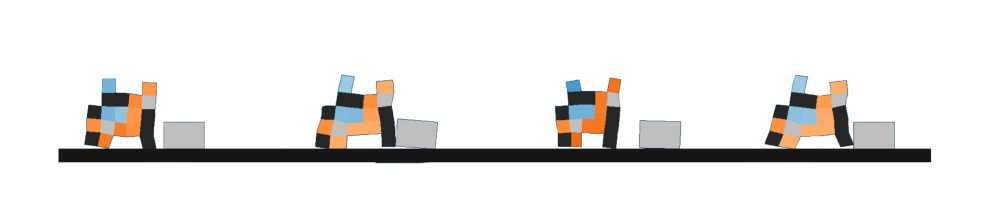
\includegraphics[scale=0.9]{images/task_pusher.pdf}
    \caption{Pusher-v0}
    \label{fig:task_pusher}
\end{figure}


\subsubsection{Carrier-v0}
The goal in this task is to carry a box, initialized above the individual, as far as possible.\\
The reward is $R = R_1 + R_2$, where $R_1$ is the score obtained according to the positive x direction motion of both the robot $r$ and the box $b$, and $R_2$ is a penalty applied when when the box falls below a certain height:
\[R_1 = 0.5 \cdot \Delta p^r_x + 0.5 \cdot \Delta p^b_x\]

\[R_2 =\begin{cases}
        0 & \text{if } p^b_y \geq t_y\\
        10 \cdot \Delta p^b_y & \text{otherwise}
    \end{cases}
    \]
where $t_y$ is the height threshold to determine whether to apply the penalty.\\
Just as in the other tasks described, the robot gets a one-time reward of 1 for successfully reaching the end of the terrain.\\
The observation space has dimension $S \in R^{2n+6}$, and is formed by concatenating vectors $v^r$, $p^b - p^r$, $v^b$, $c^r$, with lengths 2, 2, 2, $2n$ respectively.

\begin{figure}[H]
    \centering
    
\includegraphics[scale=0.9]{images/task_carrier.pdf}
    \caption{Carrier-v0}
    \label{fig:task_carrier}
\end{figure}

\newpage
      \chapter{Controller optimization}
\label{cha:controller_optimization}

Co-optimization has a key role in evolving individuals.
Some morphologies are clearly more suitable than others for some tasks, but a poorly developed controller can compromise the performance even of the fittest bodies.\\
This chapter analyzes how performances of individuals vary according to the level of optimization given to the controller.\\
Note that the results here proposed, as in the rest of the work, are obtained by averaging over the results of six experiments with different seeds. The MAP-Elites parameters applied in this experiments, and in the following ones, are shown in Table \ref{tab:me_parameters}

\begin{table}[h]
    \centering
    \begin{tabular}{|ll|}
        \hline
        \textbf{parameter name} & \textbf{value}\\
        \hline
        map\_shape &  (10, 10)\\
        num\_init & 500\\
        num\_mutated &  1500\\
        batch\_size & 28\\
        mutation\_rate & 0.1\\
        num\_attempts & 50\\
    \hline
    \end{tabular}
    \caption{MAP-Elites main parameters}
    \label{tab:me_parameters}
\end{table}

\section{Controller episodes}
The controller is optimized using PPO algorithm, as introduced in Chapter \ref{cha:chapter1}. Being an on-policy algorithm, it considers batch of data using the current policy to evaluate the reward, therefore the fitness value can vary in relation to the size of evaluation interval considered.\\
This section proposes a comparison of experiments in which the controller of the individuals is optimized using 40 or 60 episodes, to show how this choice can affect soft robot evolution.
Simulations are run in the walking environment with MAP-Elites algorithm, introduced in Chapter \ref{cha:chapter1}.

\subsection{Activity}
Being a quality diversity algorithm, MAP-Elites aims at promoting diversity.\\
After the first generation of randomly sampled morphologies, individuals are picked from the map and mutated, with no concern for their fitness.\\
Given these premises, we expect that working on the controller should not affect the choice of the individuals to evaluate and, consequently, the bins visited.

Figure \ref{fig:activity_map} shows a comparison of the activity maps, grids showing how many times a cell has been overwritten; the brighter is the color of a cell, the more its value has been overwritten.
As shown in figure, the expectations match the obtained results: both the activity maps are widely filled, and there is not a single specific bin on which they both focus.

Figure \ref{fig:activity_trend} compares the activity trends, which describe the number of explored bins after a certain number of evaluations; since the maximum number of cells that can be visited is 100, it can be read as a percentage. Note that the trends show both the mean trend (main line) and the variance (shadowed area).
The comparison makes it even more evident: the number of bins visited, after a certain number of evaluations, is almost the same, therefore changing the number of episodes for the controller optimization does not affect the choice of individuals.

\begin{figure}[H]
    \centering
    \begin{subfigure}[b]{0.49\textwidth}
         \centering
         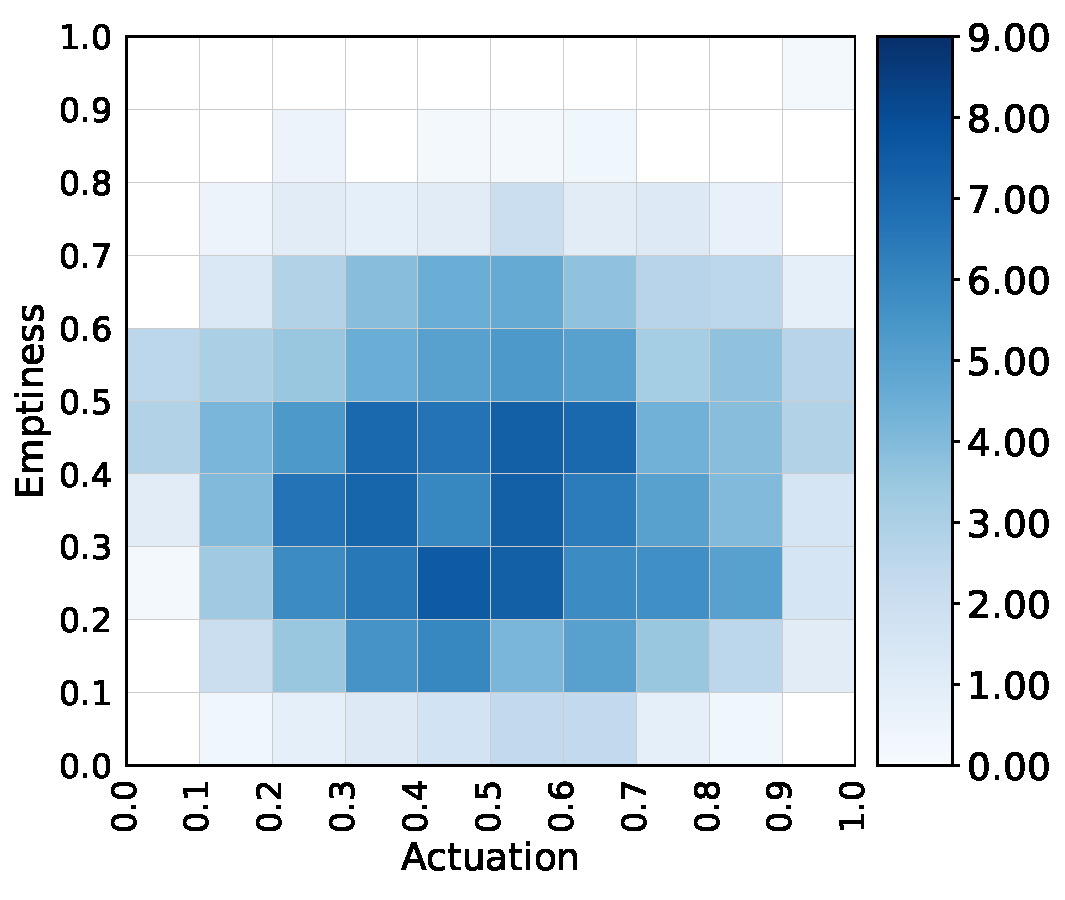
\includegraphics[scale=0.45]{images/brain_opt/walker/walker_qd_40eps_ag}
         \caption{40 episodes}
         \label{walker_ag_40}
    \end{subfigure}
    \hfill
    \begin{subfigure}[b]{0.49\textwidth}
         \centering
         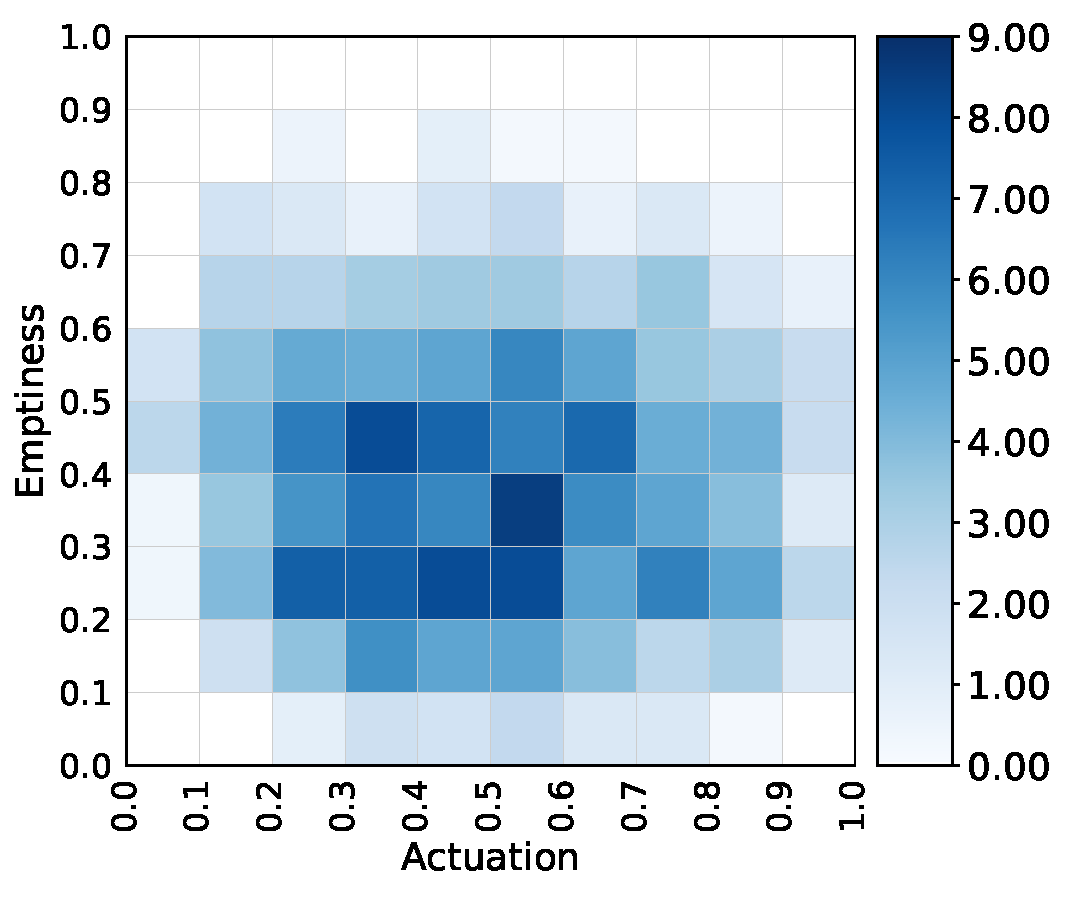
\includegraphics[scale=0.45]{images/brain_opt/walker/walker_qd_60eps_ag}
         \caption{60 episodes}
         \label{walker_ag_60}
    \end{subfigure}
    \caption{Comparison of the activity maps applying controller optimization using 40 (a) or 60 (b) episodes. The overall distribution of the visited bins is not affected.}
    \label{fig:activity_map}
\end{figure}

\begin{figure}[H]
    \centering
    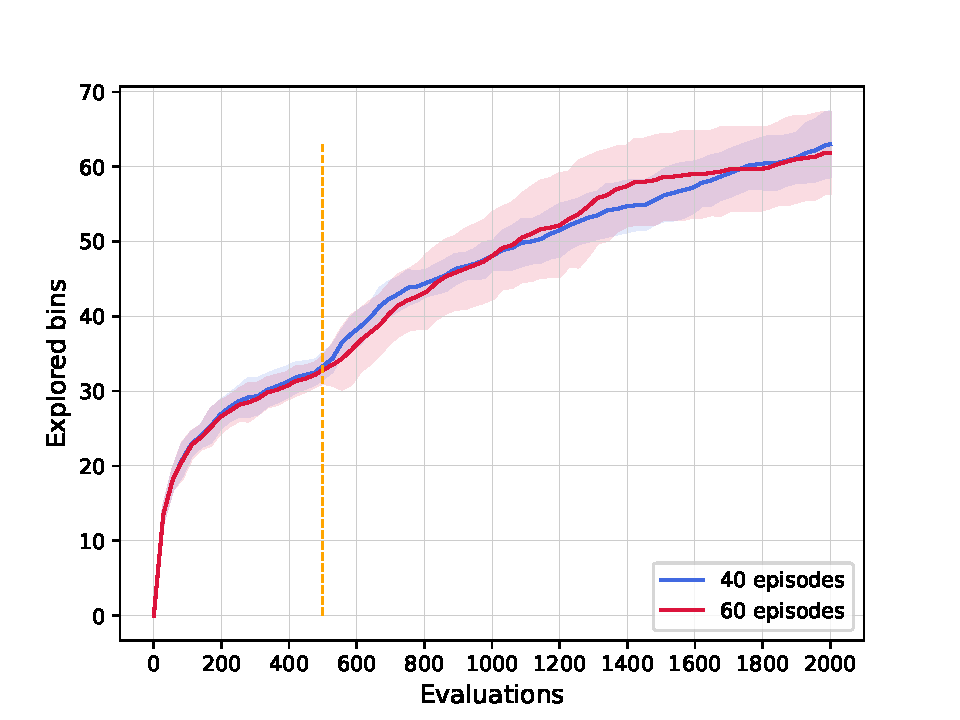
\includegraphics[scale=0.65]{images/brain_opt/walker/comp_40_60eps_at}
    \caption{Comparison of the activity trends. Changing the number of episodes for the controller optimization does not affect the activity trend, since the choice of individuals to mutate and evaluate doesn't depend on the fitness obtained}
    \label{fig:activity_trend}
\end{figure}

\subsection{Performance}
An analysis on how changing the number of episodes for the controller optimization affects the overall performance is here proposed.\\
A comparison of the fitness trends, that describe the behaviour of the best fitness value found after a certain number of evaluations, is illustrated in Figure \ref{fig:fitness_trend}, and it shows that individuals with a 60-episode-optimized controller obtain a greater reward. What is more, the 40-episodes trend has constantly greater variation, probably because of the intrinsic fitness of some morphologies: the naturally fittest bodies can get a great score even though the controller is not highly optimized, while others need to put more effort on the brain optimization to perform their best.

The effects on the fitness can be also inferred comparing the performance maps, that show for each cell the best fitness value obtained by an individual mapped to that cell; brighter cells are the ones that reached a greater fitness value.
The comparison in Figure \ref{fig:performance_map}, show that optimizing the controller with more episodes leads to greater scores all over the map, resulting in a widely spread brighter color.
This means that the more intensive controller optimization didn't affect a type of individual only, but allowed a general improvement, for all the visited cells, including the border ones.

\begin{figure}[h]
    \centering
    \begin{subfigure}[b]{0.49\textwidth}
         \centering
         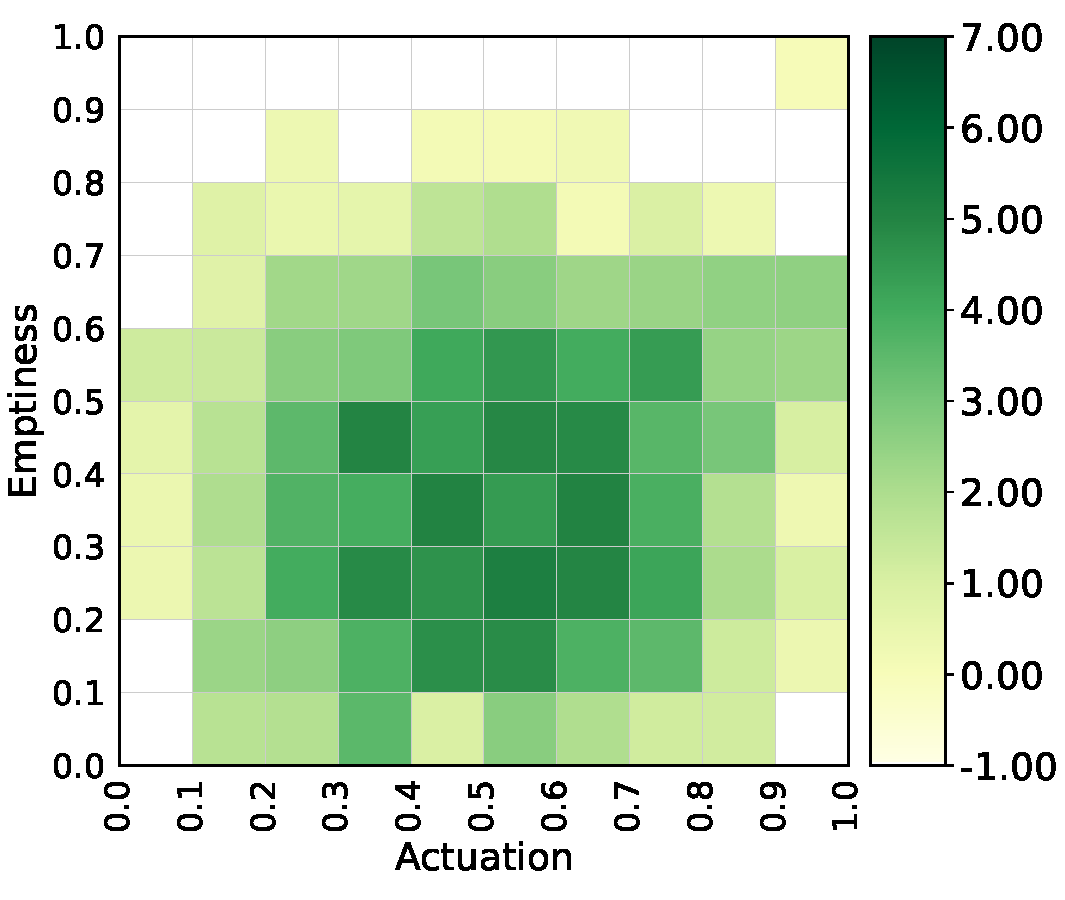
\includegraphics[scale=0.45]{images/brain_opt/walker/walker_qd_40eps_pg}
         \caption{40 episodes}
         \label{walker_pg_40}
    \end{subfigure}
    \hfill
    \begin{subfigure}[b]{0.49\textwidth}
         \centering
         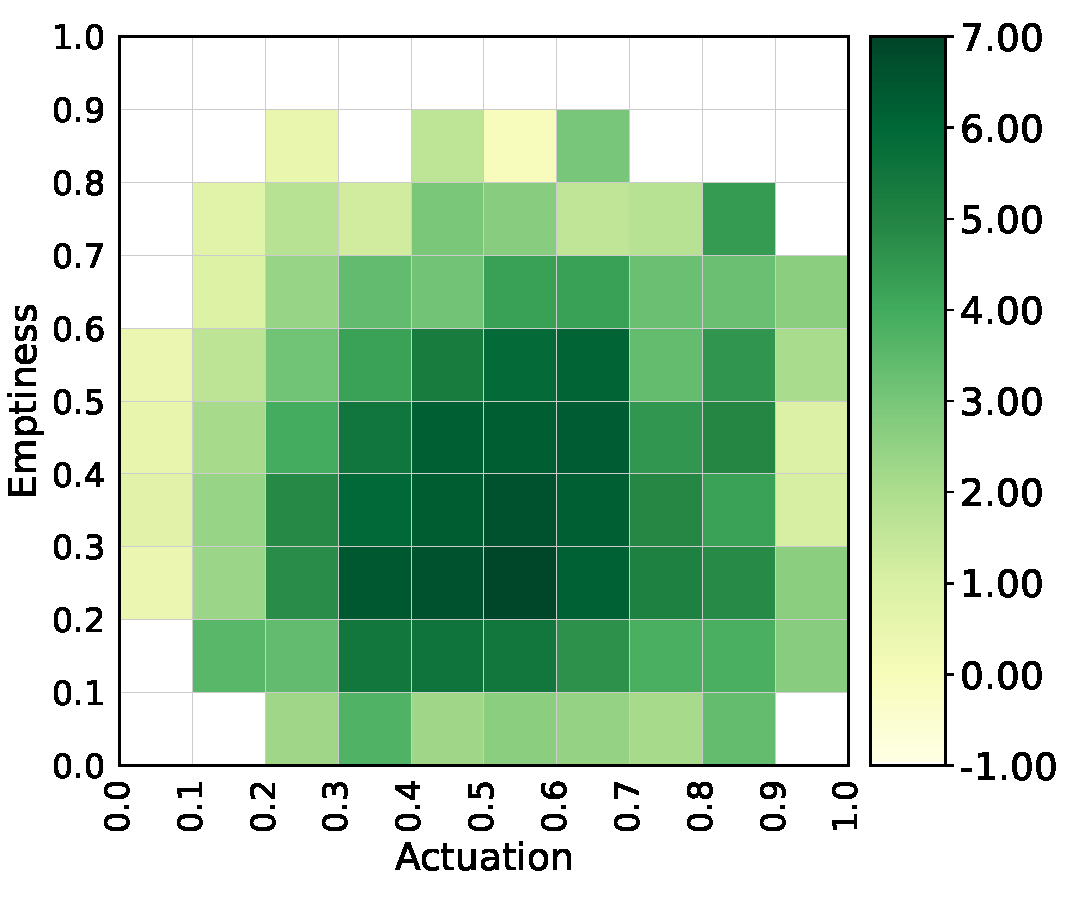
\includegraphics[scale=0.45]{images/brain_opt/walker/walker_qd_60eps_pg}
         \caption{60 episodes}
         \label{walker_pg_60}
    \end{subfigure}
    \caption{Comparison of the performance maps applying controller optimization with 40 (a) or 60 (b) episodes.
    Controller optimization highly affects the general performance of all individuals.}
    \label{fig:performance_map}
\end{figure}

\begin{figure}[h]
    \centering
    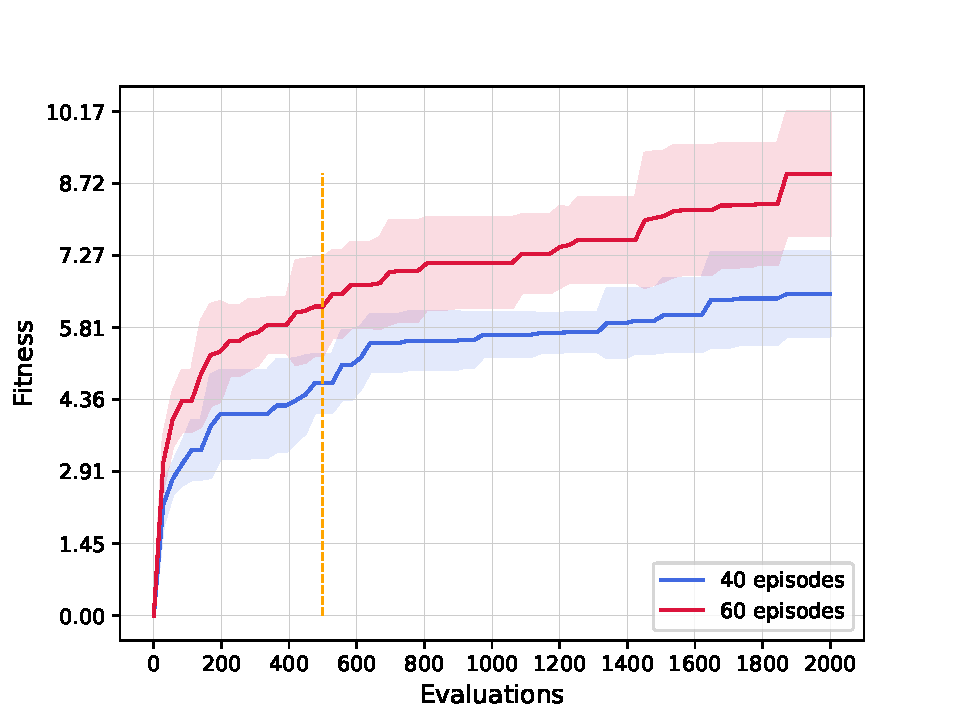
\includegraphics[scale=0.65]{images/brain_opt/walker/comp_40_60eps_ft}
    \caption{Comparison of the fitness trends. A focus on the controller optimization leads to higher fitness.}
    \label{fig:fitness_trend}
\end{figure}


\section{Conclusion}
This experiments confirmed that the controller optimization has a key role in improving the general performance of the individuals and it consequently leads to a greater reward. However, changing the number of episodes for the controller didn't affect the overall exploration of the map, since MAP-Elites chooses the individuals to mutate and evaluate from the ones stored in the map with no regard for their fitness value, as it was expected of a QD algorithm.


\newpage
      \chapter{Body optimization}
\label{cha:body_optimization}

This chapter focuses on the morphology optimization.
Selecting individuals to survive and mutate is a critical point in body optimization, therefore there are many different techniques with different goals. This chapter provides a comparison between MAP-Elites and GA, introduced in Chapter \ref{cha:chapter1}, applied to soft robot evolution.
The main difference between these algorithms is that the first one promotes diversity, while the second one allows the survival only of the best individuals per generation. Therefore it is expected that this difference affects the results.

For each experiment all the maps and trends are compared. A vertical dashed in the trend plots indicates the end of the first generation of random individuals of MAP-Elites, therefore it does not have any specific meaning in the GA application.

Since MAP-Elites is a QD algorithm, it's supposed to fill the performance map with a quite uniform color brightness. On the contrary, GA aims at optimizing the best fitness, with no regards for the body diversity.\\
For these reasons, GA is expected to achieve a better performance, but it's maps will focus only on few cells.
On the contrary MAP-Elites, since it promotes diversity, might fill the maps better and more uniformly, at the expense of the fitness value.

The tasks studied in this work are the Walker, the Pusher, and the Carrier, introduced in Chapter~\ref{cha:chapter1}.

The parameters applied to GA are shown in Table \ref{tab:ga_parameters}, while MAP-Elites parameters are the same introduced in Chapter \ref{cha:controller_optimization}; the controller optimization uses 60 episodes in both cases.

\begin{table}[H]
    \centering
    \begin{tabular}{|ll|}
        \hline
        \textbf{parameter name} & \textbf{value}\\
        \hline
        pop\_size &  100\\
        max\_evaluations & 2000\\
        x (\%) & 60-0\\
        mutation\_rate & 0.1\\
        num\_attempts & 50\\
    \hline
    \end{tabular}
    \caption{GA main parameters}
    \label{tab:ga_parameters}
\end{table}


%%%%%%%%%%%%%%%%%%%%%%%% WALKER %%%%%%%%%%%%%%%%%%%%%%%% 
\section{Walker}
The walker task is the simplest one, since the only interactions the robot has with the environment are the ones with the terrain.\\
Given these premises, the maximum fitness value is expected to be high using both the algorithms.

\subsection{Performance analysis}
A comparison of the fitness trends, shown in Figure \ref{fig:qd_ga_walker_ft}, points out that the two curves have similar shapes. GA performs slightly better since the first generations, but MAP-Elites gets very good results too.

\begin{figure}[h]
    \centering
    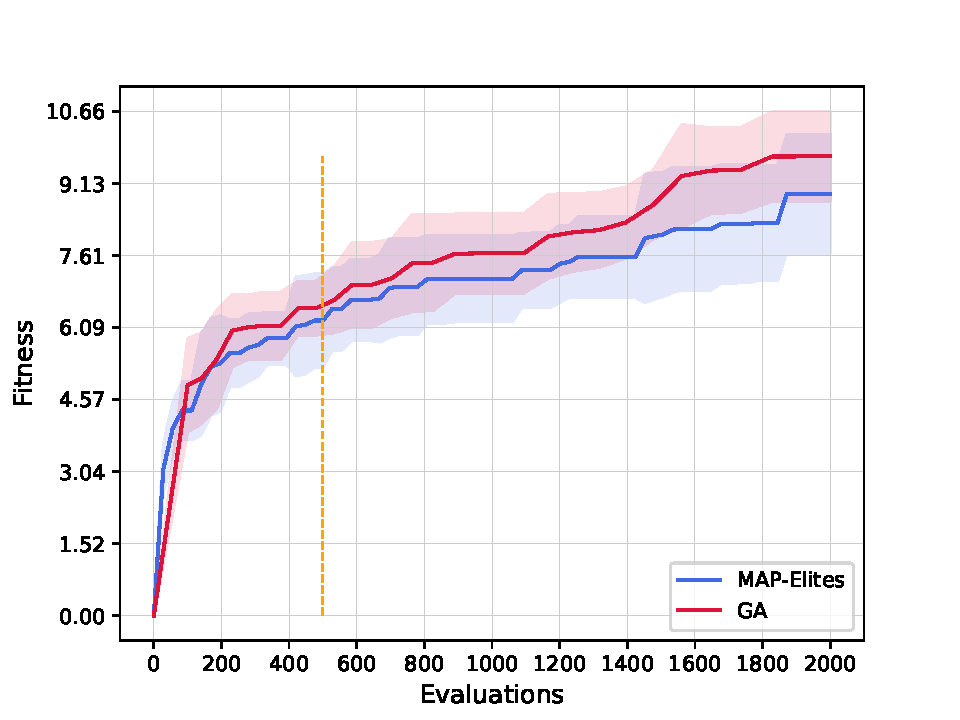
\includegraphics[scale=0.65]{images/body_opt/comp_qd_ga_w_ft}
    \caption{Walker task fitness trend comparison. The two algorithms reach high fitness values, and the two curves have similar shapes.}
    \label{fig:qd_ga_walker_ft}
\end{figure}

The performance grids in Figure \ref{fig:qd_ga_walker_pg} confirm that the two algorithms reach good fitness values, since they both have dark green coloured cells.\\
The main difference is that MAP-Elites widely fills the map, and the color is uniformly distributed, with a slightly brighter color in the center, whereas the GA map highlights that its best fitness values converge to a specific bin, and a noticeable color difference exists between that cell and the border ones.

\begin{figure}[h]
    \centering
    \begin{subfigure}[b]{0.49\textwidth}
         \centering
         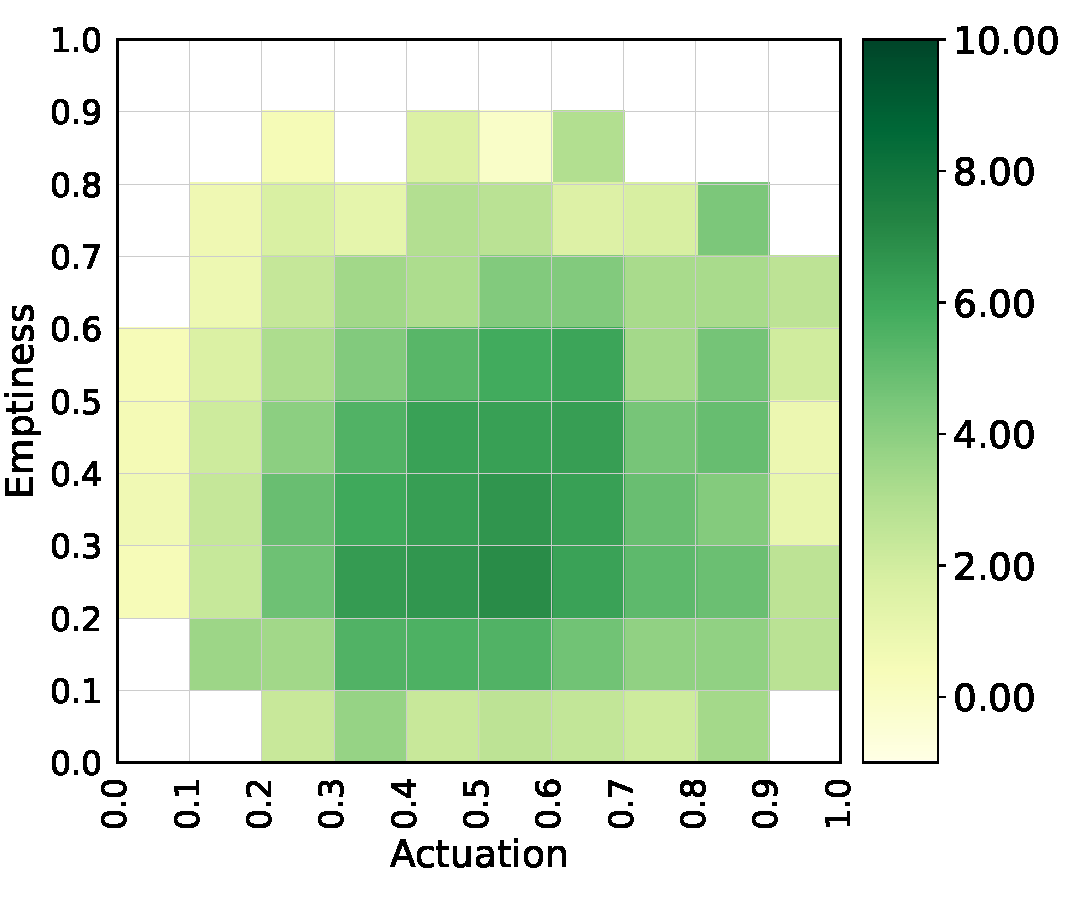
\includegraphics[scale=0.45]{images/body_opt/walker_qd_pg}
         \caption{MAP-Elites}
    \end{subfigure}
    \hfill
    \begin{subfigure}[b]{0.49\textwidth}
         \centering
         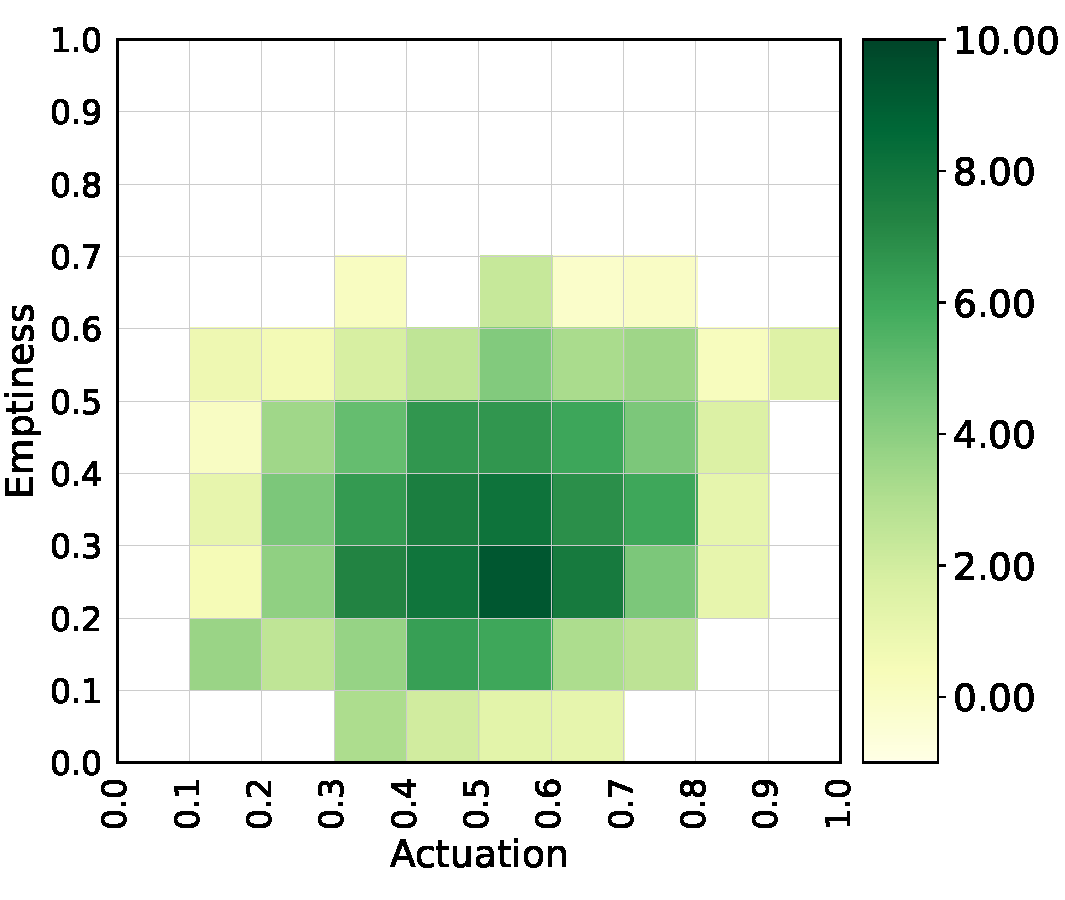
\includegraphics[scale=0.45]{images/body_opt/walker_ga_pg}
         \caption{GA}
    \end{subfigure}
    \caption{Walker task performance grid comparison. MAP-Elites (a) fills the map quite uniformly; GA (b) converges to a specific bin.}
    \label{fig:qd_ga_walker_pg}
\end{figure}

\subsection{Activity analysis}
An analysis on the activity maps, shown in Figure \ref{fig:qd_ga_walker_ag}, underlines the different approaches of the two design optimization algorithms.

The GA map shows that the value of a specific cell has been overwritten multiple times. It is not by chance that the most active cell is also the one with the best performance (in relation to Figure \ref{fig:qd_ga_walker_pg}): this is due to the fact the only goal of GA is to always get better performing individuals, selecting, and then mutating, the best ones at the end of each generation.

\begin{figure}[H]
    \centering
    \begin{subfigure}[b]{0.49\textwidth}
         \centering
         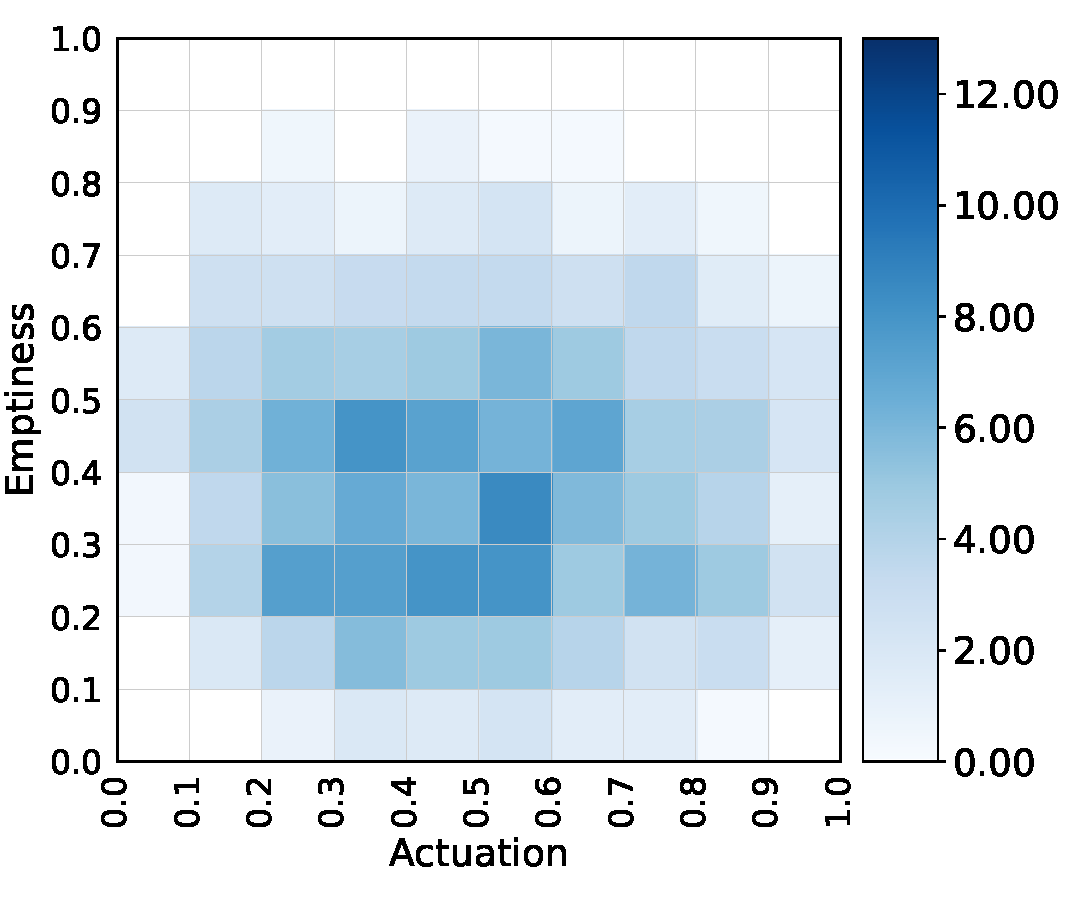
\includegraphics[scale=0.45]{images/body_opt/walker_qd_ag}
         \caption{MAP-Elites}
    \end{subfigure}
    \hfill
    \begin{subfigure}[b]{0.49\textwidth}
         \centering
         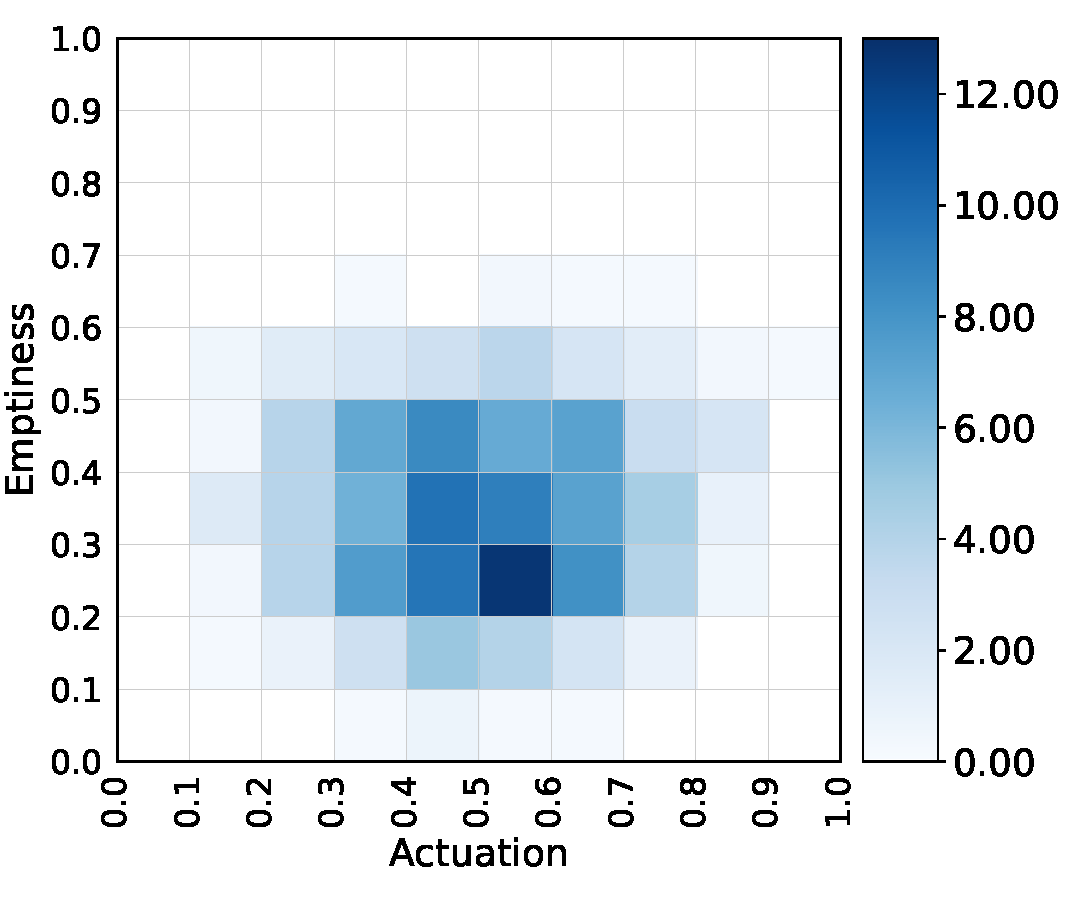
\includegraphics[scale=0.45]{images/body_opt/walker_ga_ag}
         \caption{GA}
    \end{subfigure}
    \caption{Walker task activity grid comparison. MAP-Elites (a) fills the map widely and uniformly; GA (b) focuses on few cells and converges to a specific bin, that coincides with the one with the best fitness value.}
    \label{fig:qd_ga_walker_ag}
\end{figure}

On the contrary, MAP-Elites activity map is uniform and it's not correlated to the performance map, confirming that the algorithm is not focused on the mere best fitness achievement. However, the cells in the center have a darker colour in comparison with the ones in the border. This is mainly because there's less chance of having individuals with feature values at the end of the domain.

Thanks to the activity trends in Figure \ref{fig:qd_ga_walker_at}, it is possible to analyze the number of explored bins in the map in relation to the number of evaluated individuals.\\
The curves of the two algorithms have similar shapes for the first 500 evaluations, which is the number of individuals that MAP-Elites generates randomly. After this threshold, the number of bins explored by MAP-Elites increases highly and quite constantly, whereas GA continues a much slower rise.
This confirms that promoting diversity also means promoting exploration of the feature domains.

\begin{figure}[h]
    \centering
    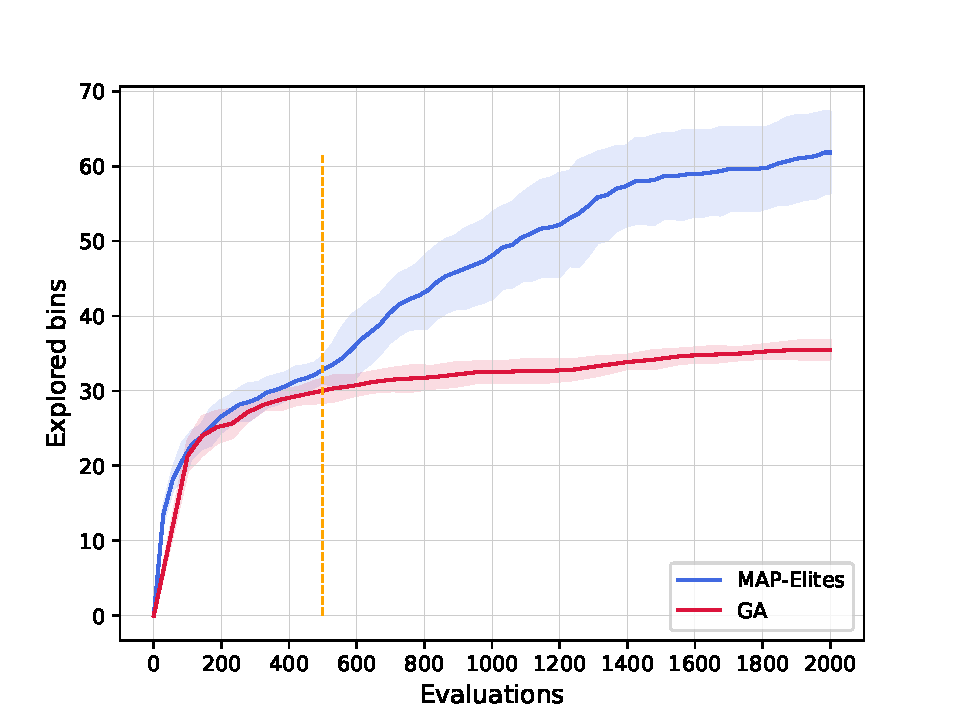
\includegraphics[scale=0.65]{images/body_opt/comp_qd_ga_w_at}
    \caption{Walker task activity trend comparison. After a generation of randomly generated bodies, MAP-Elites continuously explores different cells. GA, after the first few generations, has a much slower rise, since it focuses on few cells.}
    \label{fig:qd_ga_walker_at}
\end{figure}

\subsection{Top designs}
The morphologies of the best performing individuals emphasize the different approaches of the two algorithms.\\
Using GA, the best individuals per generation survive and new individuals can be generated by a mutation of those who survived. Therefore, the resulting top designs are very similar, as shown in Figure \ref{fig:ga_walker_topdesigns}.\\
MAP-Elites is a QD algorithm, therefore it promotes diversity: the best performing individuals, shown in Figure \ref{fig:qd_walker_topdesigns}, have different morphologies.\\
However, most of the top designs obtained by the two algorithms have a great number of horizontal actuators and they have grown two legs, which is what allows them to walk; this interesting result highlights once again the strong connection with biology, since they resemble natural creatures, even though they had no prior knowledge.

\begin{figure}[H]
    \centering
    \begin{tabular}{cccccc}
    \rule{0pt}{9ex}  
    
\includegraphics[scale=0.1]{images/top_designs/walker/ga/ga3_gen29_ind0} &
    
\includegraphics[scale=0.1]{images/top_designs/walker/ga/ga3_gen29_ind1} &
    
\includegraphics[scale=0.1]{images/top_designs/walker/ga/ga3_gen29_ind2} &
    
\includegraphics[scale=0.1]{images/top_designs/walker/ga/ga3_gen29_ind3} &
    
\includegraphics[scale=0.1]{images/top_designs/walker/ga/ga3_gen29_ind4} &
    
\includegraphics[scale=0.1]{images/top_designs/walker/ga/ga3_gen29_ind5} \\
    \hline \rule{0pt}{9ex}  
    
\includegraphics[scale=0.1]{images/top_designs/walker/ga/ga5_gen29_ind0} &
    
\includegraphics[scale=0.1]{images/top_designs/walker/ga/ga5_gen29_ind1} &
    
\includegraphics[scale=0.1]{images/top_designs/walker/ga/ga5_gen29_ind2} &
    
\includegraphics[scale=0.1]{images/top_designs/walker/ga/ga5_gen29_ind3} &
    
\includegraphics[scale=0.1]{images/top_designs/walker/ga/ga5_gen29_ind4} &
    
\includegraphics[scale=0.1]{images/top_designs/walker/ga/ga5_gen29_ind5}\\
    \hline \rule{0pt}{9ex}  
    
\includegraphics[scale=0.1]{images/top_designs/walker/ga/ga6_gen29_ind0} &
    
\includegraphics[scale=0.1]{images/top_designs/walker/ga/ga6_gen29_ind1} &
    
\includegraphics[scale=0.1]{images/top_designs/walker/ga/ga6_gen29_ind2} &
    
\includegraphics[scale=0.1]{images/top_designs/walker/ga/ga6_gen29_ind3} &
    
\includegraphics[scale=0.1]{images/top_designs/walker/ga/ga6_gen29_ind4} &
    
\includegraphics[scale=0.1]{images/top_designs/walker/ga/ga6_gen29_ind5}\\
\end{tabular}

    \caption{GA best performing morphologies on the walker task in three different experiments. For each experiment, top designs look very similar.}
    \label{fig:ga_walker_topdesigns}
\end{figure}

\begin{figure}[H]
    \centering
    \begin{tabular}{cccccc}
    \rule{0pt}{9ex}  
    
\includegraphics[scale=0.1]{images/top_designs/walker/map_elites/exp3/0_ind1668.png} &
    
\includegraphics[scale=0.1]{images/top_designs/walker/map_elites/exp3/1_ind1839.png} &
    
\includegraphics[scale=0.1]{images/top_designs/walker/map_elites/exp3/2_ind563.png} &
    
\includegraphics[scale=0.1]{images/top_designs/walker/map_elites/exp3/3_ind1860.png} &
    
\includegraphics[scale=0.1]{images/top_designs/walker/map_elites/exp3/4_ind1297.png} &
    
\includegraphics[scale=0.1]{images/top_designs/walker/map_elites/exp3/5_ind911.png}\\
    \hline \rule{0pt}{9ex}  
    
\includegraphics[scale=0.1]{images/top_designs/walker/map_elites/exp1/0_ind1650.png} &
    
\includegraphics[scale=0.1]{images/top_designs/walker/map_elites/exp1/1_ind1719.png} &
    
\includegraphics[scale=0.1]{images/top_designs/walker/map_elites/exp1/2_ind1462.png} &
    
\includegraphics[scale=0.1]{images/top_designs/walker/map_elites/exp1/3_ind1481.png} &
    
\includegraphics[scale=0.1]{images/top_designs/walker/map_elites/exp1/4_ind1559.png} &
    
\includegraphics[scale=0.1]{images/top_designs/walker/map_elites/exp1/5_ind1270.png}\\
    \hline \rule{0pt}{9ex}  
    
\includegraphics[scale=0.1]{images/top_designs/walker/map_elites/exp4/0_ind1535.png} &
    
\includegraphics[scale=0.1]{images/top_designs/walker/map_elites/exp4/1_ind1775.png} &
    \includegraphics[scale=0.1]{images/top_designs/walker/map_elites/exp4/2_ind1692.png} &
    \includegraphics[scale=0.1]{images/top_designs/walker/map_elites/exp4/3_ind1759.png} &
    \includegraphics[scale=0.1]{images/top_designs/walker/map_elites/exp4/4_ind1183.png}&
    \includegraphics[scale=0.1]{images/top_designs/walker/map_elites/exp4/5_ind165.png}\\
\end{tabular}
    \caption{MAP-Elites best performing morphologies on the walker task in three different experiments. The algorithm produced well-performing individuals with various designs.}
    \label{fig:qd_walker_topdesigns}
\end{figure}


%%%%%%%%%%%%%%%%%%%%%%%% PUSHER %%%%%%%%%%%%%%%%%%%%%%%% 
\section{Pusher}
In this environment, the goal is to push an object as far as possible. To do so, individuals must also learn how to walk. The object can't be simply thrown, because a penalty is applied according to its distance from the body.

\subsection{Performance analysis}
An analysis on the performance map, in Figure \ref{fig:qd_ga_pusher_pg}, shows that GA finds well-performing individuals that are mapped on few close cells. On the contrary, MAP-Elites widely fills the map, and shows that even boundary cells, poorly touched by GA, can lead to interesting results.

The fitness trend comparison in Figure \ref{fig:qd_ga_pusher_ft} shows that the behaviour of the two algorithms in finding the best fitness value is very similar, especially for the first evaluations. This means that the two of them, after the same amount of evaluations, found vary similar, fitness values.\\
After further evaluations, they both continued their growth; the reduction of standard deviation in GA confirms that its behaviour is quite regular.

\begin{figure}[H]
    \centering
    \begin{subfigure}[b]{0.49\textwidth}
         \centering
         \includegraphics[scale=0.45]{images/brain_opt/pusher/pusher_qd_pg}
         \caption{MAP-Elites}
    \end{subfigure}
    \hfill
    \begin{subfigure}[b]{0.49\textwidth}
         \centering
         \includegraphics[scale=0.45]{images/brain_opt/pusher/pusher_ga_pg}
         \caption{GA}
    \end{subfigure}
    \caption{Pusher-v0 performance map comparison. GA (b) best performing individuals converge to few cells, while MAP-Elites map (a) is more uniform.}
    \label{fig:qd_ga_pusher_pg}
\end{figure}

\begin{figure}[H]
    \centering
    \includegraphics[scale=0.65]{images/brain_opt/pusher/comp_qd_ga_p_ft}
    \caption{Pusher-v0. Fitness trend comparison. The two algorithms have a similar behaviour, but GA gets higher fitness values.}
    \label{fig:qd_ga_pusher_ft}
\end{figure}

\subsection{Activity analysis}
As it was expected, the activity map of GA, shown in Figure \ref{fig:qd_ga_pusher_ag} focuses only on few cells. More specifically, border cells are the less visited, while it greatly focuses on the cells with the most common feature values. It's not by choice that the most overwritten cells are the one with the best fitness values.\\
On the contrary, MAP-Elites doesn't focus on few cells only. Its central area is more coloured, but there is not a small region that stands out. Also, its most overwritten cells do not coincide with the best performing ones, as it can be seen comparing the activity and the performance maps.

Comparing the number of explored bins behaviour, in Figure \ref{fig:qd_ga_pusher_at}, it is possible to distinguish two different moments. For the first 500 evaluations, the two lines almost coincide. The morphologies evaluated by MAP-Elites in this stage are randomly sampled, so it's an exploration stage. After further evaluations, GA continues a slow increase, that becomes steady at around 35\% of explored bins. On the contrary, MAP-Elites continues its rise to about 60\% of explored bins, almost twice as GA.\\
Also, the low standard deviation in the activity trend of GA confirms that this is a common behaviour for the algorithm, which focuses on the performance with no regards for the map exploration.

\begin{figure}[H]
    \centering
    \begin{subfigure}[b]{0.49\textwidth}
         \centering
         \includegraphics[scale=0.45]{images/brain_opt/pusher/pusher_qd_ag}
         \caption{MAP-Elites}
    \end{subfigure}
    \hfill
    \begin{subfigure}[b]{0.49\textwidth}
         \centering
         \includegraphics[scale=0.45]{images/brain_opt/pusher/pusher_ga_ag}
         \caption{GA}
    \end{subfigure}
    \caption{Pusher-v0 activity map comparison. GA (b) focuses on few cells only, while MAP-Elites map (a) is widely and more uniformely explored.}
    \label{fig:qd_ga_pusher_ag}
\end{figure}

\begin{figure}[H]
    \centering
    \includegraphics[scale=0.65]{images/brain_opt/pusher/comp_qd_ga_p_at}
    \caption{Pusher-v0. Activity trend comparison. After a generation of randomly generated bodies, MAP-Elites continuously explores different cells. GA, after the first few generations, has a much slower rise, since it focuses on few cells}
    \label{fig:qd_ga_pusher_at}
\end{figure}

\subsection{Top designs}
The designs of the best performing individuals behave differently according to the algorithm applied. The best individuals per generation found by GA are the ones to survive, and they can mutate to generate offspring. This is why the top designs look very similar, as shown in Figure \ref{fig:ga_pusher_topdesigns}. On the contrary, MAP-Elites promotes diversity, so the top designs obtained, in Figure \ref{fig:qd_pusher_topdesigns}, have different morphologies.
Since the pusher task also had the implicit goal of leaning to walk, most of the the individuals obtained grew legs.

\begin{figure}[H]
    \centering
    \begin{tabular}{cccccc}
    \rule{0pt}{9ex}  
    \includegraphics[scale=0.1]{images/top_designs/pusher/ga/exp1/gen29_ind0} &
    \includegraphics[scale=0.1]{images/top_designs/pusher/ga/exp1/gen29_ind1} &
    \includegraphics[scale=0.1]{images/top_designs/pusher/ga/exp1/gen29_ind2} &
    \includegraphics[scale=0.1]{images/top_designs/pusher/ga/exp1/gen29_ind3} &
    \includegraphics[scale=0.1]{images/top_designs/pusher/ga/exp1/gen29_ind4} &
    \includegraphics[scale=0.1]{images/top_designs/pusher/ga/exp1/gen29_ind5} \\
    \hline \rule{0pt}{9ex}  
    \includegraphics[scale=0.1]{images/top_designs/pusher/ga/exp3/gen29_ind0} &
    \includegraphics[scale=0.1]{images/top_designs/pusher/ga/exp3/gen29_ind1} &
    \includegraphics[scale=0.1]{images/top_designs/pusher/ga/exp3/gen29_ind2} &
    \includegraphics[scale=0.1]{images/top_designs/pusher/ga/exp3/gen29_ind3} &
    \includegraphics[scale=0.1]{images/top_designs/pusher/ga/exp3/gen29_ind4} &
    \includegraphics[scale=0.1]{images/top_designs/pusher/ga/exp3/gen29_ind5} \\
    \hline \rule{0pt}{9ex}  
    \includegraphics[scale=0.1]{images/top_designs/pusher/ga/exp5/gen29_ind0} &
    \includegraphics[scale=0.1]{images/top_designs/pusher/ga/exp5/gen29_ind1} &
    \includegraphics[scale=0.1]{images/top_designs/pusher/ga/exp5/gen29_ind2} &
    \includegraphics[scale=0.1]{images/top_designs/pusher/ga/exp5/gen29_ind3} &
    \includegraphics[scale=0.1]{images/top_designs/pusher/ga/exp5/gen29_ind4} &
    \includegraphics[scale=0.1]{images/top_designs/pusher/ga/exp5/gen29_ind5} \\
\end{tabular}

    \caption{GA best performing morphologies on the pusher task in three different experiments. For each experiment, top designs look very similar.}
    \label{fig:ga_pusher_topdesigns}
\end{figure}

\begin{figure}[H]
    \centering
    \begin{tabular}{cccccc}
    \rule{0pt}{9ex}  
    \includegraphics[scale=0.1]{images/top_designs/pusher/map_elites/exp6/0_ind1672.png} &
    \includegraphics[scale=0.1]{images/top_designs/pusher/map_elites/exp6/1_ind1573.png} &
    \includegraphics[scale=0.1]{images/top_designs/pusher/map_elites/exp6/2_ind1648.png} &
    \includegraphics[scale=0.1]{images/top_designs/pusher/map_elites/exp6/3_ind1796.png} &
    \includegraphics[scale=0.1]{images/top_designs/pusher/map_elites/exp6/4_ind1924.png} &
    \includegraphics[scale=0.1]{images/top_designs/pusher/map_elites/exp6/5_ind1516.png}\\
    \hline \rule{0pt}{9ex}  
    \includegraphics[scale=0.1]{images/top_designs/pusher/map_elites/exp4/0_ind1682.png} &
    \includegraphics[scale=0.1]{images/top_designs/pusher/map_elites/exp4/1_ind1334.png} &
    \includegraphics[scale=0.1]{images/top_designs/pusher/map_elites/exp4/2_ind1704.png} &
    \includegraphics[scale=0.1]{images/top_designs/pusher/map_elites/exp4/3_ind1961.png} &
    \includegraphics[scale=0.1]{images/top_designs/pusher/map_elites/exp4/4_ind1818.png} &
    \includegraphics[scale=0.1]{images/top_designs/pusher/map_elites/exp4/5_ind1698.png}\\
    \hline \rule{0pt}{9ex}  
    \includegraphics[scale=0.1]{images/top_designs/pusher/map_elites/exp2/0_ind1707.png} &
    \includegraphics[scale=0.1]{images/top_designs/pusher/map_elites/exp2/1_ind986.png} &
    \includegraphics[scale=0.1]{images/top_designs/pusher/map_elites/exp2/2_ind1731.png} &
    \includegraphics[scale=0.1]{images/top_designs/pusher/map_elites/exp2/3_ind1288.png} &
    \includegraphics[scale=0.1]{images/top_designs/pusher/map_elites/exp2/4_ind1057.png} &
    \includegraphics[scale=0.1]{images/top_designs/pusher/map_elites/exp2/5_ind1410.png}\\
\end{tabular}
    \caption{MAP-Elites best performing morphologies on the pusher task in three different experiments. The algorithm produced well-performing individuals with various designs.}
    \label{fig:qd_pusher_topdesigns}
\end{figure}


%%%%%%%%%%%%%%%%%%%%%%%% CARRIER %%%%%%%%%%%%%%%%%%%%%%%%
\section{Carrier}
In this task, the goal is to carry an object as far as possible.\\
The individuals trained in this task are supposed to learn how to walk and how to carry a box initialized in front of
them.

\subsection{Performance analysis}
A comparison of the performance grids in Figure \ref{fig:qd_ga_carrier_pg} show that MAP-Elites fills the map more widely than GA.\\
GA gets a higher best fitness value, and the distribution of color in its cells shows that the individuals with a good performance converge to few cells only. However, focusing on few cells only precludes it to find well-performing individuals in other map areas. On the contrary, MAP-Elites, exploring the map, found well performing individuals even on the boundary cells, never explored by GA.\\
Since a penalty is applied when the object falls under a certain height, some individuals stored in the map have a negative fitness value.

The fitness trend comparison in Figure \ref{fig:qd_ga_carrier_ft}, shows that GA has higher best-fitness values after all evaluation intervals. Even though they sometimes get very close, MAP-Elites never obtains a higher best-fitness value. This is mainly because GA focuses on obtaining the best individual, therefore it selects its best performing robots to survive and, potentially, mutate. On the contrary, the selection of individuals to mutate in MAP-Elites is not driven by their fitness value.

\begin{figure}[H]
    \centering
    \includegraphics[scale=0.65]{images/brain_opt/carrier/comp_qd_ga_c_ft}
    \caption{Carrier-v0. Fitness trend comparison.
    The two algorithms have a similar behaviour, but GA gets higher fitness values.}
    \label{fig:qd_ga_carrier_ft}
\end{figure}

\begin{figure}[H]
    \centering
    \begin{subfigure}[b]{0.49\textwidth}
         \centering
        \includegraphics[scale=0.45]{images/brain_opt/carrier/carrier_qd_pg}
         \caption{MAP-Elites}
    \end{subfigure}
    \hfill
    \begin{subfigure}[b]{0.49\textwidth}
         \centering
         \includegraphics[scale=0.45]{images/brain_opt/carrier/carrier_ga_pg}
         \caption{GA}
    \end{subfigure}
    \caption{Carrier-v0 performance map comparison. GA (b) best performing individuals converge to few cells, while MAP-Elites map (a) is more uniform.}
    \label{fig:qd_ga_carrier_pg}
\end{figure}

\subsection{Activity analysis}
The activity trend comparison in Figure \ref{fig:qd_ga_carrier_at} highlights the different approaches the two algorithms have in exploring the map.\\
GA has a rapid growth in the first evaluations, but then it remains stable at around 35\% of explored bins.
On the contrary, MAP-Elites has a gradual rise for all the experiment, leading to an almost doubled number of explored cells, compared to GA.

\begin{figure}[h]
    \centering
    \includegraphics[scale=0.65]{images/brain_opt/carrier/comp_qd_ga_c_at}
    \caption{Carrier-v0. Activity trend comparison.
    After a generation of randomly generated bodies, MAP-Elites continuously explores different cells. GA, after the first few generations, has a much slower rise, since it focuses on few cells}
    \label{fig:qd_ga_carrier_at}
\end{figure}

This is mainly because GA tends to focus on few cells, as illustrated in Figure \ref{fig:qd_ga_carrier_ag}, and trying to get better fitness values from individuals with the same features becomes always harder.\\
The activity map of MAP-Elites is widely filled, and picking from the many cells with lower fitness values, as previously analyzed from Figure \ref{fig:qd_ga_carrier_pg}, increases the chance to overwrite them.

\begin{figure}[H]
    \centering
    \begin{subfigure}[b]{0.49\textwidth}
         \centering
         \includegraphics[scale=0.45]{images/brain_opt/carrier/carrier_qd_ag}
         \caption{MAP-Elites}
    \end{subfigure}
    \hfill
    \begin{subfigure}[b]{0.49\textwidth}
         \centering
         \includegraphics[scale=0.45]{images/brain_opt/carrier/carrier_ga_ag}
         \caption{GA}
    \end{subfigure}
    \caption{Carrier-v0 activity map comparison. GA (b) focuses on few cells only, while MAP-Elites map (a) is widely and more uniformely explored.}
    \label{fig:qd_ga_carrier_ag}
\end{figure}

\subsection{Top designs}
GA and MAP-Elites are designed with different goals: the first focuses on obtaining the best performance, the last one on the diversity. This difference is reflected on the resulting top designs. While individuals found by GA, Figure \ref{fig:ga_carrier_topdesigns} look evidently very similar, the ones obtained by MAP-Elites, shown in Figure \ref{fig:qd_carrier_topdesigns}, don't.
However, the two algorithms agree on the need of extra space above the individual to carry the box. Even though it was not a constraint of the task, all the best performing carriers have empty voxels above them, surrounded by few non-empty voxels to keep them from falling forward or backwards.

\begin{figure}[H]
    \centering
    \begin{tabular}{cccccc}
    \rule{0pt}{9ex}  
    \includegraphics[scale=0.1]{images/top_designs/carrier/ga/exp1/gen29_ind0} &
    \includegraphics[scale=0.1]{images/top_designs/carrier/ga/exp1/gen29_ind1} &
    \includegraphics[scale=0.1]{images/top_designs/carrier/ga/exp1/gen29_ind2} &
    \includegraphics[scale=0.1]{images/top_designs/carrier/ga/exp1/gen29_ind3} &
    \includegraphics[scale=0.1]{images/top_designs/carrier/ga/exp1/gen29_ind4} &
    \includegraphics[scale=0.1]{images/top_designs/carrier/ga/exp1/gen29_ind5} \\
    \hline \rule{0pt}{9ex}  
    \includegraphics[scale=0.1]{images/top_designs/carrier/ga/exp2/gen29_ind0} &
    \includegraphics[scale=0.1]{images/top_designs/carrier/ga/exp2/gen29_ind1} &
    \includegraphics[scale=0.1]{images/top_designs/carrier/ga/exp2/gen29_ind2} &
    \includegraphics[scale=0.1]{images/top_designs/carrier/ga/exp2/gen29_ind3} &
    \includegraphics[scale=0.1]{images/top_designs/carrier/ga/exp2/gen29_ind4} &
    \includegraphics[scale=0.1]{images/top_designs/carrier/ga/exp2/gen29_ind5} \\
    \hline \rule{0pt}{9ex}  
    \includegraphics[scale=0.1]{images/top_designs/carrier/ga/exp5/gen29_ind0} &
    \includegraphics[scale=0.1]{images/top_designs/carrier/ga/exp5/gen29_ind1} &
    \includegraphics[scale=0.1]{images/top_designs/carrier/ga/exp5/gen29_ind2} &
    \includegraphics[scale=0.1]{images/top_designs/carrier/ga/exp5/gen29_ind3} &
    \includegraphics[scale=0.1]{images/top_designs/carrier/ga/exp5/gen29_ind4} &
    \includegraphics[scale=0.1]{images/top_designs/carrier/ga/exp5/gen29_ind5} \\
\end{tabular}

    \caption{GA best performing morphologies on the carrier task in three different experiments. For each experiment, top designs look very similar.}
    \label{fig:ga_carrier_topdesigns}
\end{figure}

\begin{figure}[H]
    \centering
    \begin{tabular}{cccccc}
    \rule{0pt}{9ex}  
    \includegraphics[scale=0.1]{images/top_designs/carrier/map_elites/exp5/0_ind1365.png} &
    \includegraphics[scale=0.1]{images/top_designs/carrier/map_elites/exp5/1_ind1454.png} &
    \includegraphics[scale=0.1]{images/top_designs/carrier/map_elites/exp5/2_ind1424.png} &
    \includegraphics[scale=0.1]{images/top_designs/carrier/map_elites/exp5/3_ind1916.png} &
    \includegraphics[scale=0.1]{images/top_designs/carrier/map_elites/exp5/4_ind1631.png} &
    \includegraphics[scale=0.1]{images/top_designs/carrier/map_elites/exp5/5_ind1981.png}\\
    \hline \rule{0pt}{9ex}  
    \includegraphics[scale=0.1]{images/top_designs/carrier/map_elites/exp1/0_ind1505.png} &
    \includegraphics[scale=0.1]{images/top_designs/carrier/map_elites/exp1/1_ind869.png} &
    \includegraphics[scale=0.1]{images/top_designs/carrier/map_elites/exp1/2_ind1867.png} &
    \includegraphics[scale=0.1]{images/top_designs/carrier/map_elites/exp1/3_ind1113.png} &
    \includegraphics[scale=0.1]{images/top_designs/carrier/map_elites/exp1/4_ind1744.png} &
    \includegraphics[scale=0.1]{images/top_designs/carrier/map_elites/exp1/5_ind937.png}\\
    \hline \rule{0pt}{9ex}  
    \includegraphics[scale=0.1]{images/top_designs/carrier/map_elites/exp3/0_ind1737.png} &
    \includegraphics[scale=0.1]{images/top_designs/carrier/map_elites/exp3/1_ind712.png} &
    \includegraphics[scale=0.1]{images/top_designs/carrier/map_elites/exp3/2_ind862.png} &
    \includegraphics[scale=0.1]{images/top_designs/carrier/map_elites/exp3/3_ind1541.png} &
    \includegraphics[scale=0.1]{images/top_designs/carrier/map_elites/exp3/4_ind984.png} &
    \includegraphics[scale=0.1]{images/top_designs/carrier/map_elites/exp3/5_ind205.png}\\
\end{tabular}
    \caption{MAP-Elites best performing morphologies on the carrier task in three different experiments. The algorithm produced well-performing individuals with various designs.}
    \label{fig:qd_carrier_topdesigns}
\end{figure}



\section{Conclusion}
The Genetic Algorithm finds greater fitness values but, after a short initial exploration of the map, it focuses only on few cells. The most explored bins correspond to the ones with the greatest fitness, and this is because the fittest individuals survive through generations, therefore they are more likely to be selected and mutated, to generate new individuals.
As a consequence, the top individuals have very similar designs.\\
On the contrary, MAP-Elites widely explores the map and evaluates individuals with different feature values. Even though the central area in the map is usually the most visited, due to the higher chance of having bodies with medium feature values, boundary cells are not disregarded, and they can lead to interesting results. 
Since this algorithm promotes diversity, the individuals with the best fitness have various morphologies.\\
Even though the best fitness found by MAP-Elites algorithm is always lower than the one reached by GA, it does not disappoint. This results confirm that QD algorithms can find well performing individuals, that might be rejected by other reward-oriented algorithms like GA.\\
However, the two algorithms evolved robot bodies with some similarities: they grew legs or evolved space to carry an object, according to their task goal, resembling natural creatures even with no prior knowledge.


\newpage
      \chapter{Multitasking}
\label{cha:multitasking}

The goal of soft robotics is to generate a new category of robots, inspired by nature and designed to perform well on dynamic and unpredictable environments.\\
This chapter analyzes the behaviour of map-elites best performing individuals in tasks they where not designed for.
For each experiment, the fittest individuals in a certain task, which are the ones stored in the final map, have been trained in a new task.

Since the walker task observation space is different from the ones of the other two environments it is compared with, validating individuals using both the structures and the controllers already optimized and stored is impossible.
For this reason, the morphologies of the best individuals have been used with no optimization, and the controller has been re-optimized in the new environment.

Nevertheless, in the carrier and pusher tasks individuals have also been evaluated using both the body and the controller already optimized in the original task. This has been possible since the observation space of the two tasks is the same.


\section{Preliminary considerations}
Figure \ref{fig:task_comparison} displays the fitness trends of experiments in the three tasks, using MAP-Elites to optimize the design, and PPO to optimize the controller.\\
The three trends are not comparable because of the different reward definition of the three tasks.

The pusher and the carrier are expected to be good walkers, since they both have the implicit goal of learning how to walk, other than interacting with an object. The opposite is not true: even though an individual is a good walker, he might be incapable of interacting with an object, since it only learned how to walk. It might not disappoint as a pusher, as a good morphology with a strong front leg might allow it to oppose to the box resistance. The same cannot be said for carrying a box, as it requires a good conformation at the top of the robot, to prevent the box from falling.

\begin{figure}
    \centering
    \begin{subfigure}[b]{0.3\textwidth}
        \centering
        \includegraphics[scale=0.35]{images/multitasking/ft_walker.pdf}
        \caption{Walker}
    \end{subfigure}
    \begin{subfigure}[b]{0.3\textwidth}
        \centering
        \includegraphics[scale=0.35]{images/multitasking/ft_pusher.pdf}
        \caption{Pusher}
    \end{subfigure}
    \begin{subfigure}[b]{0.3\textwidth}
        \centering
        \includegraphics[scale=0.35]{images/multitasking/ft_carrier.pdf}
        \caption{Carrier}
    \end{subfigure}
    \caption{Fitness trend in the three tasks.}
    \label{fig:task_comparison}
\end{figure}


\section{Task performance comparison}
Is an individual who has only learnt how to walk able to push or carry an object? Can a pusher (carrier) carry (push) an object as far as possible? How well can pushers and carriers walk?
This section tries to answer to these questions by providing the performance map generated in a task and the ones obtained by training the same individuals in a different environment.

Note that the reward definition vary according to the task, therefore the results obtained by evaluating in different environments are not comparable.
For more details about the reward definition of the three tasks, pleas refer to Chapter \ref{cha:chapter1}.

Figure \ref{fig:walker_multitask} shows the performance maps generated by optimizing the controller of the best walker designs in the walking task itself (Map \ref{walker_a}), in the pusher and carrier task (Maps \ref{walker_b} and \ref{walker_c} respectively).\\
The obtained maps highlights that walkers might be good pushers, however the overall fitness in the carrier task is poor.\\
The results meet the expectations, since the ability of walking might help to push an object forward, but it doesn't provide any knowledge on how to carry a box.

The results of best pusher designs trained in the three tasks are shown in Figure \ref{fig:pusher_multitask}. These individuals are well able of pushing an object, for which they had been designed for, and walking forward; however, once again, they get poor results in the carrier task. The maps obtained in the first two tasks are very similar, and this is because walking is an implicit goal while learning to push a box forward.

The best carrier designs obtain interesting, but not excellent, results in the walking and pushing environment, as shown in Figure \ref{fig:carrier_multitask}. Map \ref{carrier_c} highlights that the best performing individuals in the carrier task are the ones for which the body and the controller have both been trained in that same environment.

%%%% WALKER %%%%
\begin{figure}
    \centering
    \begin{subfigure}[b]{0.3\textwidth}
         \centering
         \includegraphics[scale=0.3]{images/multitasking/walker.pdf}
         \caption{Walker}
         \label{walker_a}
     \end{subfigure}
     \hfill
     \begin{subfigure}[b]{0.3\textwidth}
         \centering
         \includegraphics[scale=0.3]{images/multitasking/walker_p.pdf}
         \caption{Pusher}
         \label{walker_b}
     \end{subfigure}
     \hfill
     \begin{subfigure}[b]{0.3\textwidth}
         \centering
         \includegraphics[scale=0.3]{images/multitasking/walker_c.pdf}
         \caption{carrier}
         \label{walker_c}
     \end{subfigure}
    \caption{Walker designs trained in the walker (a), pusher (b), carrier (c) task.
    The maps can be compared for the fitness distribution, however the obtained fitness cannot be compared, since its definition is different in the three tasks.}
    \label{fig:walker_multitask}
\end{figure}

%%%% PUSHER %%%
\begin{figure}
    \centering
    \begin{subfigure}[b]{0.3\textwidth}
         \centering
         \includegraphics[scale=0.3]{images/multitasking/pusher_w.pdf}
         \caption{Walker}
         \label{pusher_a}
    \end{subfigure}
    \hfill
    \begin{subfigure}[b]{0.3\textwidth}
         \centering
         \includegraphics[scale=0.3]{images/multitasking/pusher.pdf}
         \caption{Pusher}
         \label{pusher_b}
    \end{subfigure}
    \hfill
    \begin{subfigure}[b]{0.3\textwidth}
         \centering
         \includegraphics[scale=0.3]{images/multitasking/pusher_c.pdf}
         \caption{Carrier}
         \label{pusher_c}
    \end{subfigure}
    \caption{Pusher designs trained in the walker (a), pusher (b), carrier (c) task.
    The maps can be compared for the fitness distribution, however the obtained fitness cannot be compared, since its definition is different in the three tasks.}
    \label{fig:pusher_multitask}
\end{figure}

%%% CARRIER %%%
\begin{figure}
    \centering
    \begin{subfigure}[b]{0.3\textwidth}
         \centering
         \includegraphics[scale=0.3]{images/multitasking/carrier_w.pdf}
         \caption{Walker}
         \label{carrier_a}
    \end{subfigure}
    \hfill
    \begin{subfigure}[b]{0.3\textwidth}
         \centering
         \includegraphics[scale=0.3]{images/multitasking/carrier_p.pdf}
         \caption{Pusher}
         \label{carrier_b}
    \end{subfigure}
    \hfill
    \begin{subfigure}[b]{0.3\textwidth}
         \centering
         \includegraphics[scale=0.3]{images/multitasking/carrier.pdf}
         \caption{Carrier}
         \label{carrier_c}
    \end{subfigure}
    \caption{Carrier designs trained in the walker (a), pusher (b), carrier (c) task.
    The maps can be compared for the fitness distribution, however the obtained fitness cannot be compared, since its definition is different in the three tasks.}
    \label{fig:carrier_multitask}
\end{figure}


Table \ref{tab:results} provides the numerical results of these experiments.
Each row defines where the designs of the individuals have been optimized, the columns refer to the environment on which the individuals have been evaluated.

Each cell indicates the mean and the standard deviation of the designs best performing in the environment in row, trained in the task in column.
The value of each cell has been computed by considering all the individuals in the final map of six experiments, launched with different seeds. The respective mediated maps are the ones shown in Figures \ref{fig:walker_multitask}, \ref{fig:pusher_multitask}, \ref{fig:carrier_multitask}.

The table confirms that for each task the greatest rewards are obtained by the individuals for which the body and the controller have been optimized in that same environment.

Note the the results in row are not comparable, since each task has its own definition of reward, defined in Chapter \ref{cha:chapter1}.

\begin{table}[h]
    \centering
    \begin{tabular}{r|c|c|c|}
         & Walker task & Pusher task & Carrier task \\
         \hline
        Walker & $3.913 \pm 2.21$ & $ 1.7\pm1.391 $ & $-0.602 \pm 0.938$\\
        Pusher & $  2.297\pm1.989 $ & $2.713 \pm 1.533$ & $-0.424 \pm 0.975$ \\
        Carrier & $ 1.481\pm1.634 $ & $ 1.275\pm1.237 $ & $0.801 \pm 1.286$ \\
        \hline
    \end{tabular}
    \caption{Comparison of task performance.
    Each row defines where the bodies have been optimized; each column refers to the environment on which the controllers have been trained, and where the individuals have been evaluated.
    Each cell indicates the mean and standard deviation.
    Please note the the results in row are not comparable since each task defines its own reward.}
    \label{tab:results}
\end{table}



\section{Validating or training in a new task}
The carrier and pusher task have the same observation space, therefore it's possible to use both the body and the controller optimized in an environment on the other task.

%%% CARRIER %%%
The best performing carriers get a higher fitness value in the pusher task if their controller is trained in the new environment, as shown in Figure \ref{fig:carrier_val_tr}.\\
The first row in Table \ref{tab:carrier_pusher_results} confirms that the mean fitness is greater when the controller is optimized in the new environment, but it also shows that it has a greater standard deviation.

\begin{figure}[H]
    \centering
    \begin{subfigure}[b]{0.49\textwidth}
         \centering
         \includegraphics[scale=0.4]{images/multitasking/carrier_val_p.pdf}
         \caption{Validation}
    \end{subfigure}
    \hfill
    \begin{subfigure}[b]{0.49\textwidth}
         \centering
         \includegraphics[scale=0.4]{images/multitasking/carrier_tr_p.pdf}
         \caption{Controller training}
    \end{subfigure}
    \caption{Performances of the best carrier designs in the pusher task.  The the performances of individuals are improved when controllers are trained in the new task (b), compared with the validation only (a).}
    \label{fig:carrier_val_tr}
 \end{figure}

\begin{figure}[h]
    \centering
    \begin{subfigure}[b]{0.49\textwidth}
         \centering
         \includegraphics[scale=0.4]{images/multitasking/pusher_val_c.pdf}
         \caption{Validation}
    \end{subfigure}
    \hfill
    \begin{subfigure}[b]{0.49\textwidth}
         \centering
         \includegraphics[scale=0.4]{images/multitasking/pusher_tr_c.pdf}
         \caption{Controller training}
    \end{subfigure}
    \caption{Performances of the best pusher designs in the carrier task. The comparison shows that simply validating individuals (a) gets better results than training controllers (b) in the new task.}
    \label{fig:pusher_val_tr}
 \end{figure}
 
%%% PUSHER %%%
Figure \ref{fig:pusher_val_tr} provides a comparison of the best pusher designs validating and optimizing the controller in the carrier task.\\
Contrary to the considerations for the carrier designs in the pusher task, the two maps highlight that the validated individuals perform better than the ones whose controller has been trained in the new task.\\
The results are confirmed by computing the mean of the fitness, as shown in the second row in Table \ref{tab:carrier_pusher_results}. However, the table also points out that not optimizing the controller leads to a greater standard deviation.\\
The greater result with no further optimization is due to the pushers walking ability: since a component of the carrier task reward consists of the position of the robot, this ability allows it to get a good fitness value, despite the behaviour of the box.
 
\begin{table}[H]
    \centering
    \begin{tabular}{|l|c|c|}
    \cline{2-3}
    \multicolumn{1}{c|}{} & \multicolumn{1}{c|}{validation} & \multicolumn{1}{c|}{optimization}\\
    \hline
        carrier designs & $ 0.54 \pm 0.84 $ & $ 1.275 \pm 1.237 $ \\
        \hline
        pusher designs & $ 0.124 \pm 1.369 $ & $ -0.424 \pm 0.975 $ \\
    \hline
    \end{tabular}
    \caption{Carrier and pusher multitask experiments.
    Mean and standard deviation for the experiments with validation only or with the controller optimization in the new task.
    The first row shows the results of the best carrier designs in the pusher task, the second row refers to the best pusher designs in the carrier task.}
    \label{tab:carrier_pusher_results}
\end{table}


\section{Conclusion}
This chapter introduced some considerations about using the same designs in various tasks.

The best results in each environment are obtained when the body and the controller are both optimized in the same task, confirming that the robot co-optimization is strongly connected to the environment definition.

The pusher and carrier tasks showed that it's also possible to perform well on a new task even with no controller re-optimization; however, since it doesn't provide excellent results, further analysis might provide interesting and surely more precise information.

The reward definition of the task on which individuals are evaluated greatly affects the results.
About this, it was shown that the best pusher designs can get a great reward in the carrier task even with no controller optimization in the new environment, due to their ability to walk, which increases the final reward value in spite of the penalty applied for dropping the box.

\newpage
      \chapter{Conclusions}
\label{cha:coclusion}

This work provided an overview of soft robot evolution using Evolution Gym benchmark.\\
Soft robotics is a promising brand new robotic research field.
The main feature of soft robots, which is their deformability and adaptability to complex and unpredictable environments, makes them an interesting subject. 
Not only are they bio-inspired, but also they will have many future bio-related applications, and their malleability and adaptability will lead to an enhanced human-machine interaction.

A focus on the controller optimization showed that it has a key role in soft robot evolution, since it allows all the individuals to perform their best, even the ones with a disadvantaged morphology.

A comparison of two design algorithms, GA and MAP-Elites, showed that focusing on the mere fitness goal does lead to greater fitness values, but it generates similar bodies, precluding from exploring new potentially well-fitting morphologies. On the contrary, focusing on diversity allows the evaluation of very different robot designs, and it leads to only slightly lower performances.

One of the main reasons why soft robots are considered a promising field is their flexibility and adaptability, and therefore their potential application in different environments.
This work revealed that even though the best results are obtained when both the controller and the body are optimized in the same task, it's also possible to get good results in a new environment simply by re-training the controller.\\
It was also shown that in some environments it's also possible to use the already optimized controller; this avoids the optimization costs and, in some cases, turned out to be even more effective.
However, these results depend on the reward definition, and further experiments might take to more accurate results.

The robot bodies evolved autonomously often resembled existing natural creatures, even with no prior knowledge: for instance, they grew legs and set space to carry an object, according to the goal of the task they have been trained on. This demonstrates once again the strong connection that persists between artificial intelligence and biology.

Nevertheless, this work only focused on three easy tasks. The benchmark used proposes a great variety of tasks of different difficulty, therefore it would be interesting to extend the study of soft robot evolution to more complex environments.\\
The design optimization was limited to two evolutionary algorithms, but many other exist and might lead to interesting results.\\
What is more, only two body-related features were considered, the actuation and the emptiness, therefore a deeper study might analyze other features, like the energy consumption, relevant for future applications.

This work only provided an overview of soft robot evolution, but many encouraging aspects emerged yet. This is a promising field that deserves to be explored, and further studies will surely take steps towards an enhanced human-machine interaction.

\newpage


    \endgroup

    % bibliografia in formato bibtex
    % aggiunta del capitolo nell'indice
    \addcontentsline{toc}{chapter}{Bibliography}
    % stile con ordinamento alfabetico in funzione degli autori
    \bibliographystyle{plain}
    \bibliography{biblio}


\end{document}
